% Options for packages loaded elsewhere
\PassOptionsToPackage{unicode}{hyperref}
\PassOptionsToPackage{hyphens}{url}
\PassOptionsToPackage{dvipsnames,svgnames,x11names}{xcolor}
%
\documentclass[
  11pt,
  article]{jss}

\usepackage{amsmath,amssymb}
\usepackage{iftex}
\ifPDFTeX
  \usepackage[T1]{fontenc}
  \usepackage[utf8]{inputenc}
  \usepackage{textcomp} % provide euro and other symbols
\else % if luatex or xetex
  \usepackage{unicode-math}
  \defaultfontfeatures{Scale=MatchLowercase}
  \defaultfontfeatures[\rmfamily]{Ligatures=TeX,Scale=1}
\fi
\usepackage{lmodern}
\ifPDFTeX\else  
    % xetex/luatex font selection
\fi
% Use upquote if available, for straight quotes in verbatim environments
\IfFileExists{upquote.sty}{\usepackage{upquote}}{}
\IfFileExists{microtype.sty}{% use microtype if available
  \usepackage[]{microtype}
  \UseMicrotypeSet[protrusion]{basicmath} % disable protrusion for tt fonts
}{}
\makeatletter
\@ifundefined{KOMAClassName}{% if non-KOMA class
  \IfFileExists{parskip.sty}{%
    \usepackage{parskip}
  }{% else
    \setlength{\parindent}{0pt}
    \setlength{\parskip}{6pt plus 2pt minus 1pt}}
}{% if KOMA class
  \KOMAoptions{parskip=half}}
\makeatother
\usepackage{xcolor}
\setlength{\emergencystretch}{3em} % prevent overfull lines
\setcounter{secnumdepth}{-\maxdimen} % remove section numbering
% Make \paragraph and \subparagraph free-standing
\ifx\paragraph\undefined\else
  \let\oldparagraph\paragraph
  \renewcommand{\paragraph}[1]{\oldparagraph{#1}\mbox{}}
\fi
\ifx\subparagraph\undefined\else
  \let\oldsubparagraph\subparagraph
  \renewcommand{\subparagraph}[1]{\oldsubparagraph{#1}\mbox{}}
\fi


\providecommand{\tightlist}{%
  \setlength{\itemsep}{0pt}\setlength{\parskip}{0pt}}\usepackage{longtable,booktabs,array}
\usepackage{calc} % for calculating minipage widths
% Correct order of tables after \paragraph or \subparagraph
\usepackage{etoolbox}
\makeatletter
\patchcmd\longtable{\par}{\if@noskipsec\mbox{}\fi\par}{}{}
\makeatother
% Allow footnotes in longtable head/foot
\IfFileExists{footnotehyper.sty}{\usepackage{footnotehyper}}{\usepackage{footnote}}
\makesavenoteenv{longtable}
\usepackage{graphicx}
\makeatletter
\def\maxwidth{\ifdim\Gin@nat@width>\linewidth\linewidth\else\Gin@nat@width\fi}
\def\maxheight{\ifdim\Gin@nat@height>\textheight\textheight\else\Gin@nat@height\fi}
\makeatother
% Scale images if necessary, so that they will not overflow the page
% margins by default, and it is still possible to overwrite the defaults
% using explicit options in \includegraphics[width, height, ...]{}
\setkeys{Gin}{width=\maxwidth,height=\maxheight,keepaspectratio}
% Set default figure placement to htbp
\makeatletter
\def\fps@figure{htbp}
\makeatother

\usepackage{booktabs}
\usepackage{longtable}
\usepackage{array}
\usepackage{multirow}
\usepackage{wrapfig}
\usepackage{float}
\usepackage{pdflscape}
\usepackage{tabu}
\usepackage{threeparttable}
\usepackage{threeparttablex}
\usepackage[normalem]{ulem}
\usepackage[utf8]{inputenc}
\usepackage{makecell}
\usepackage{xcolor}
\usepackage{placeins}


\newtheorem{definition}{Definition}
\usepackage{orcidlink,thumbpdf,lmodern}

\newcommand{\class}[1]{`\code{#1}'}
\newcommand{\fct}[1]{\code{#1()}}
\makeatletter
\@ifpackageloaded{tcolorbox}{}{\usepackage[skins,breakable]{tcolorbox}}
\@ifpackageloaded{fontawesome5}{}{\usepackage{fontawesome5}}
\definecolor{quarto-callout-color}{HTML}{909090}
\definecolor{quarto-callout-note-color}{HTML}{0758E5}
\definecolor{quarto-callout-important-color}{HTML}{CC1914}
\definecolor{quarto-callout-warning-color}{HTML}{EB9113}
\definecolor{quarto-callout-tip-color}{HTML}{00A047}
\definecolor{quarto-callout-caution-color}{HTML}{FC5300}
\definecolor{quarto-callout-color-frame}{HTML}{acacac}
\definecolor{quarto-callout-note-color-frame}{HTML}{4582ec}
\definecolor{quarto-callout-important-color-frame}{HTML}{d9534f}
\definecolor{quarto-callout-warning-color-frame}{HTML}{f0ad4e}
\definecolor{quarto-callout-tip-color-frame}{HTML}{02b875}
\definecolor{quarto-callout-caution-color-frame}{HTML}{fd7e14}
\makeatother
\makeatletter
\makeatother
\makeatletter
\makeatother
\makeatletter
\@ifpackageloaded{caption}{}{\usepackage{caption}}
\AtBeginDocument{%
\ifdefined\contentsname
  \renewcommand*\contentsname{Table of contents}
\else
  \newcommand\contentsname{Table of contents}
\fi
\ifdefined\listfigurename
  \renewcommand*\listfigurename{List of Figures}
\else
  \newcommand\listfigurename{List of Figures}
\fi
\ifdefined\listtablename
  \renewcommand*\listtablename{List of Tables}
\else
  \newcommand\listtablename{List of Tables}
\fi
\ifdefined\figurename
  \renewcommand*\figurename{Figure}
\else
  \newcommand\figurename{Figure}
\fi
\ifdefined\tablename
  \renewcommand*\tablename{Table}
\else
  \newcommand\tablename{Table}
\fi
}
\@ifpackageloaded{float}{}{\usepackage{float}}
\floatstyle{ruled}
\@ifundefined{c@chapter}{\newfloat{codelisting}{h}{lop}}{\newfloat{codelisting}{h}{lop}[chapter]}
\floatname{codelisting}{Listing}
\newcommand*\listoflistings{\listof{codelisting}{List of Listings}}
\makeatother
\makeatletter
\@ifpackageloaded{caption}{}{\usepackage{caption}}
\@ifpackageloaded{subcaption}{}{\usepackage{subcaption}}
\makeatother
\makeatletter
\makeatother
\ifLuaTeX
  \usepackage{selnolig}  % disable illegal ligatures
\fi
\IfFileExists{bookmark.sty}{\usepackage{bookmark}}{\usepackage{hyperref}}
\IfFileExists{xurl.sty}{\usepackage{xurl}}{} % add URL line breaks if available
\urlstyle{same} % disable monospaced font for URLs
\hypersetup{
  pdftitle={Making, Updating, and Querying Causal Models using CausalQueries},
  pdfauthor={Till Tietz; Lily Medina; Georgiy Syunyaev; Macartan Humphreys},
  colorlinks=true,
  linkcolor={blue},
  filecolor={Maroon},
  citecolor={Blue},
  urlcolor={Blue},
  pdfcreator={LaTeX via pandoc}}

%% -- Article metainformation (author, title, ...) -----------------------------

%% Author information
\author{Till Tietz~\orcidlink{0000-0002-2916-9059}\\WZB \And Lily
Medina\\UC Berkeley \AND Georgiy
Syunyaev~\orcidlink{0000-0002-4391-6313}\\Vanderbilt
University \And Macartan Humphreys~\orcidlink{0000-0001-7029-2326}\\WZB}
\Plainauthor{Till Tietz, Lily Medina, Georgiy Syunyaev, Macartan
Humphreys} %% comma-separated

\title{Making, Updating, and Querying Causal Models using
\texttt{CausalQueries}}
\Plaintitle{Making, Updating, and Querying Causal Models using
CausalQueries} %% without formatting

%% an abstract and keywords
\Abstract{A guide to the \proglang{R} package \texttt{CausalQueries} for
making, updating, and querying causal models}

%% at least one keyword must be supplied
\Keywords{Causal Models, Stan, Bayesian Updating}

%% publication information
%% NOTE: Typically, this can be left commented and will be filled out by the technical editor
%% \Volume{50}
%% \Issue{9}
%% \Month{June}
%% \Year{2012}
%% \Submitdate{2012-06-04}
%% \Acceptdate{2012-06-04}
%% \setcounter{page}{1}
%% \Pages{1--xx}

%% The address of (at least) one author should be given
%% in the following format:
\Address{
Till Tietz\\
IPI\\
Reichpietschufer 50\\
Berlin Germany\\
E-mail: \email{ttietz2014@gmail.com}\\
URL: \url{https://github.com/till-tietz}\\
\\~
Lily Medina\\
E-mail: \email{lily.medina@berkeley.edu}\\
URL: \url{https:/lilymedina.github.io/}\\
\\~
Georgiy Syunyaev\\
E-mail: \email{g.syunyaev@vanderbilt.edu}\\
URL: \url{https://gsyunyaev.com/}\\
\\~
Macartan Humphreys\\
E-mail: \email{macartan.humphreys@wzb.eu}\\
URL: \url{https://macartan.github.io/}\\
\\~

}

\begin{document}
\maketitle
\hypertarget{sec-intro}{%
\section{Introduction: Causal models}\label{sec-intro}}

\texttt{CausalQueries} is an \proglang{R} package that lets users make,
update, and query causal models. Users provide a statement that reports
a set of binary variables and the relations of causal ancestry between
them: which variables are direct causes of other variables, given the
other variables in the model. Once provided to \texttt{make\_model()},
\texttt{CausalQueries} generates a parameter vector that fully describes
a probability distribution over all possible types of causal relations
between variables (``causal types''), given the causal structure. Given
a prior over parameters and data over some or all nodes,
\texttt{update\_model()} deploys a Stan \citep{carpenter_stan_2017}
model in order to generate a posterior distribution over causal models.
The function \texttt{query\_model()} can then be used to ask any causal
query of the model, using either the prior distribution, the posterior
distribution, or a user-specified candidate vector of parameters.

In the next section we provide a short motivating example. We then
describe how the package relates to existing available software.
Section~\ref{sec-theory} gives an overview of the statistical model
behind the package. Section~\ref{sec-make}, Section~\ref{sec-update},
and Section~\ref{sec-query} then describe the main functionality for the
major operations using the package. We provide further computation
details in the final section.

\hypertarget{motivating-example}{%
\section{Motivating example}\label{motivating-example}}

Before providing details on package functionality we illustrate these
three core functions by showing how to use \texttt{CuasalQueries} to
replicate the analysis in \citeauthor{chickering_clinicians_1996}
\citetext{\citeyear{chickering_clinicians_1996}; \citealp[see
also][]{humphreys_integrated_2023}}. \citet{chickering_clinicians_1996}
seek to draw inference on causal effects in the presence of imperfect
compliance. We have access to an instrument \(Z\) (a randomly assigned
prescription for cholesterol medication), which is a cause of \(X\)
(treatment uptake) but otherwise unrelated to \(Y\) (cholesterol). We
imagine we are interested in three specific queries. The first is the
average causal effect of \(X\) on \(Y\). The second is the average
effect for units for which \(X=0\) and \(Y=0\). The last is the average
treatment effect for ``compliers'': units for which \(X\) responds
positively to \(Z\). Thus two of these queries are conditional queries,
with one conditional on a counterfactual quantity.

Our data on \(Z\), \(X\), and \(Y\) is complete for all units and looks,
in ``compact form,'' as follows:

\begin{verbatim}
R> data("lipids_data")
R> 
R> lipids_data
\end{verbatim}

\begin{verbatim}
#>    event strategy count
#> 1 Z0X0Y0      ZXY   158
#> 2 Z1X0Y0      ZXY    52
#> 3 Z0X1Y0      ZXY     0
#> 4 Z1X1Y0      ZXY    23
#> 5 Z0X0Y1      ZXY    14
#> 6 Z1X0Y1      ZXY    12
#> 7 Z0X1Y1      ZXY     0
#> 8 Z1X1Y1      ZXY    78
\end{verbatim}

Note that in compact form we simply record the number of units
(``count'') that display each possible pattern of outcomes on the three
variables (``event'').\footnote{The ``strategy'' column records the set
  of variables for which data has been recorded.}

With \texttt{CausalQueries}, you can create the model, input data to
update it, and then query the model for results thus:

\begin{verbatim}
R> make_model("Z -> X -> Y; X <-> Y") |>
+  update_model(lipids_data, refresh = 0) |>
+  query_model(query = "Y[X=1] - Y[X=0]",
+              given = c("All",  "X==0 & Y==0", "X[Z=1] > X[Z=0]"),
+              using = "posteriors") 
\end{verbatim}

\hypertarget{tbl-lipids}{}
\begin{table}
\caption{\label{tbl-lipids}Replication of \citet{chickering_clinicians_1996}. }\tabularnewline

\centering
\resizebox{\linewidth}{!}{
\begin{threeparttable}
\begin{tabular}{cccccc}
\toprule
query & given & mean & sd & cred.low.2.5\% & cred.high.97.5\%\\
\midrule
Y[X=1] - Y[X=0] & - & 0.56 & 0.10 & 0.38 & 0.73\\
Y[X=1] - Y[X=0] & X==0 \& Y==0 & 0.64 & 0.15 & 0.38 & 0.89\\
Y[X=1] - Y[X=0] & X[Z=1] > X[Z=0] & 0.70 & 0.05 & 0.60 & 0.80\\
\bottomrule
\end{tabular}
\begin{tablenotes}
\small
\item Rows 1 and 2 replicate results in Chickering and Pearl (1996); row 3 returns inferences for complier average effects.
\end{tablenotes}
\end{threeparttable}}
\end{table}

The output is a data frame with estimates, posterior standard
deviations, and credibility intervals. For example the data frame
produced by the code above is shown in Table~\ref{tbl-lipids}.

As we describe below, the same basic procedure of making, updating, and
querying models, can be used (up to computational constraints) for
arbitrary causal models, for different types of data structures, and for
all causal queries that can be posed of the causal model.

\hypertarget{connections-to-existing-packages}{%
\section{Connections to existing
packages}\label{connections-to-existing-packages}}

The literature on causal inference and its software ecosystem are rich
and expansive; spanning the social and natural sciences as well as
computer science and applied mathematics. In the interest of clarity we
thus briefly contextualize \texttt{CausalQueries} scope and
functionality within the subset of the causal inference domain
addressing the evaluation of causal queries on causal models encoded as
directed acyclic graphs (DAGs) or structural equation models (SEMs).
Table~\ref{tbl-software} provides an overview of relevant software and
discusses key connections, advantages and disadvantages with respect to
\texttt{CausalQueries}.

\hypertarget{tbl-software}{}
\begin{longtable}[]{@{}
  >{\raggedright\arraybackslash}p{(\columnwidth - 8\tabcolsep) * \real{0.2000}}
  >{\raggedright\arraybackslash}p{(\columnwidth - 8\tabcolsep) * \real{0.1500}}
  >{\raggedright\arraybackslash}p{(\columnwidth - 8\tabcolsep) * \real{0.1000}}
  >{\raggedright\arraybackslash}p{(\columnwidth - 8\tabcolsep) * \real{0.1500}}
  >{\raggedright\arraybackslash}p{(\columnwidth - 8\tabcolsep) * \real{0.4000}}@{}}
\caption{\label{tbl-software}Related software.}\tabularnewline
\toprule\noalign{}
\begin{minipage}[b]{\linewidth}\raggedright
Software
\end{minipage} & \begin{minipage}[b]{\linewidth}\raggedright
Source
\end{minipage} & \begin{minipage}[b]{\linewidth}\raggedright
Language
\end{minipage} & \begin{minipage}[b]{\linewidth}\raggedright
Availability
\end{minipage} & \begin{minipage}[b]{\linewidth}\raggedright
Scope
\end{minipage} \\
\midrule\noalign{}
\endfirsthead
\toprule\noalign{}
\begin{minipage}[b]{\linewidth}\raggedright
Software
\end{minipage} & \begin{minipage}[b]{\linewidth}\raggedright
Source
\end{minipage} & \begin{minipage}[b]{\linewidth}\raggedright
Language
\end{minipage} & \begin{minipage}[b]{\linewidth}\raggedright
Availability
\end{minipage} & \begin{minipage}[b]{\linewidth}\raggedright
Scope
\end{minipage} \\
\midrule\noalign{}
\endhead
\bottomrule\noalign{}
\endlastfoot
\texttt{causalnex} & \citet{beaumont_causalnex_2021} & \proglang{Python}
& pip & \begin{minipage}[t]{\linewidth}\raggedright
\begin{itemize}
\tightlist
\item
  causal structure learning
\item
  querying marginal distributions
\item
  discrete data
\end{itemize}
\end{minipage} \\
\texttt{causaloptim} & \citet{sachs_general_2023} & \proglang{R} & CRAN
& \begin{minipage}[t]{\linewidth}\raggedright
\begin{itemize}
\tightlist
\item
  bounding causal effects
\item
  non-identified queries
\item
  binary data
\end{itemize}
\end{minipage} \\
\texttt{pclag} & \citet{kalisch_causal_2012} & \proglang{R} & CRAN &
\begin{minipage}[t]{\linewidth}\raggedright
\begin{itemize}
\tightlist
\item
  causal structure learning
\item
  ATEs under linear conditional expectations and no hidden selection
\end{itemize}
\end{minipage} \\
\texttt{autobounds} & \citet{duarte_automated_2023} & \proglang{Python}
& not readily installable & \begin{minipage}[t]{\linewidth}\raggedright
\begin{itemize}
\tightlist
\item
  bounding causal effects
\item
  partial identification
\item
  DAG canonicalization
\item
  binary data
\end{itemize}
\end{minipage} \\
\end{longtable}

One of the most comprehensive pieces of software in the causal modeling
domain is \texttt{causalnex}. It provides a feature-rich and highly
optimized set of tools to learn, update and query causal models using
discrete data. While avoiding the rich model parametrization via
principal strata (nodal types) employed by \texttt{CausalQueries},
allows \texttt{causalnex} to easily handle non-binary data and scale to
large causal models; it substantially restricts the set of possible
queries that can be evaluated and prior knowledge that can be specified
on models. \texttt{causalnex} is in this sense akin to machine learning
approaches to causal inference, focusing on causal structure learning in
variable rich but potentially domain knowledge poor settings and the
evaluation of simple queries over marginal distributions on learned
DAGs. The rich model structure employed by \texttt{CausalQueries} by
contrast makes it highly suited to problems where answers to complex
causal queries are sought in relatively more domain knowledge abundant
settings.

Like \texttt{causalnex}, \texttt{pclag} places particular emphasis on
causal structure learning, utilizing the resultant DAGs to recover ATEs
across all learned markov-equivalent classes implied by observed data
that satisfy linearity of conditional expectations. This approach again
is more restrictive than \texttt{CausalQueries} in the DAGs and
particularly the queries it allows.

The software bearing the highest resemblance to \texttt{CausalQueries}
with respect to model definition are \texttt{autobounds} and
\texttt{causaloptim}. Dealing with binary causal models, their
definitions of principal strata (nodal types) and the resultant set of
causal relations on the DAG (causal types) are very close to those of
\texttt{CausalQueries}. Differences in model definition arise with
respect to disturbance terms and confounding being defined implicitly
via main nodes and edges in \texttt{CausalQueries} vs explicitly via
separate disturbance nodes in \texttt{autobounds} and
\texttt{causaloptim}. While \texttt{CausalQueries} assumes canonical
form for input DAGs, \texttt{autobounds} and \texttt{causaloptim}
facilitate canonicalization. The essential difference between the
methods; however, lies in their approach to evaluating queries.

Both \texttt{autobounds} and \texttt{causaloptim} build on seminal
approaches in \citet{balke_bounds_1997} to construct bounds of queries,
using constrained polynomial and linear optimization respectively. In
contrast, \texttt{CausalQueries} utilizes Bayesian inference to generate
a posterior over the causal model which is then queried
\citep[consistent
with][]{chickering_clinicians_1996, zhang_partial_2022}. A key
difference then is the target of inference. The polynomial and linear
programming approach to querying is in principle suited to handling
larger causal models, though given their similarity in model
parametrization, \texttt{autobounds}, \texttt{causaloptim} and
\texttt{CausalQueries} face similar constraints induced by parameter
spaces expanding rapidly with model size. The Bayesian approach to model
updating and querying holds the efficiency advantage that a model can be
updated once and queried infinitely, while expensive optimization runs
are required for each separate query in \texttt{autobounds} and
\texttt{causaloptim}.

Summarizing, the particular strength of \texttt{CausalQueries} is to
allow users to specify arbitrary DAGs, arbitrary queries over nodes in
those DAGs, and use the same canonical procedure to form Bayesian
posteriors over those queries whether or not the queries are identified.
Thus in principle if researchers are interested in learning about a
quantity like the local average treatment effect and their model in fact
satisfies the conditions in \citet{angrist_identification_1996}, then
updating will recover valid estimates even if researchers are unaware
that the local average treatment effect is identified and are ignorant
of the estimation procedure proposed by
\citet{angrist_identification_1996}.

There are two broad limitations on the sets of models handled natively
by \texttt{CausalQueries}. First \texttt{CausalQueries} is designed for
models with a relatively small number of binary nodes. Because there is
no compromise made on the space of possible causal relations implied by
a given model, the parameter space grows very rapidly with the
complexity of the causal model. The complexity also depends on the
causal structure and grows rapidly with the number of parents affecting
a given child. A chain model of the form
\(A \rightarrow B \rightarrow C \rightarrow D \rightarrow E\) has just
40 parameters. A model in which \(A, B, C, D\) are all direct ancestors
of \(E\) has \(65,544\) parameters. Moving from binary to non binary
nodes has similar effects. The restriction to binary nodes is for
computational and not conceptual reasons. In fact it is possible to
employ \texttt{CausalQueries} to answer queries from models with non
binary nodes but in general the computational costs make analysis of
these models prohibitive.\footnote{For more on computation constraints
  and strategies to update and query large models see the associated
  package \texttt{CausalQueriesTools}. The core approach used here is to
  divide large causal models into modules, update on modules and
  reassemble to pose queries.}

Second, the package is geared towards learning about populations from
samples of units that are independent of each other and are
independently randomly sampled from populations. Thus the basic set up
does not address problems of sampling, clustering, hierarchical
structures, or purposive sampling. The broader framework can however be
used for these purposes (see section 9.4 of
\citet{humphreys_integrated_2023}). The targets of inference are usually
case level quantities or population quantities and
\texttt{CausalQueries} is not well suited for estimating sample
quantities.

\hypertarget{sec-theory}{%
\section{Statistical model}\label{sec-theory}}

The core conceptual framework is described in Pearl's \emph{Causality}
\citep{pearl_causality_2009} but can be summarized as follows
\citep[using the notation proposed in][]{humphreys_integrated_2023}:

\begin{definition}
  
  A ``\textbf{causal model}'' is:
  \begin{enumerate}
    \item an ordered collection of ``endogenous nodes" $Y = \{Y_1, Y_2, \dots, Y_n\}$
    \item an ordered collection of ``exogenous nodes" $\Theta = \{\theta^{Y_1}, \theta^{Y_1}, \dots, \theta^{Y_n}\}$
    \item a collection of functions $F = \{f_{Y_1}, f_{Y_2}, \dots, f_{Y_n}\}$ specifying, for each $j$, how outcome $y_j$ depends on $\theta_j$ and realizations of endogenous nodes prior to $j$.
    \item a probability distribution over $\Theta$, $\lambda$.
  \end{enumerate}
  
\end{definition}

By default, \texttt{CausalQueries} takes endogenous nodes to be
binary.\footnote{\texttt{CausalQueries} can be used also to analyse non
  binary data though with a cost of greatly increased complexity. See
  section 9.4.1 of \citet{humphreys_integrated_2023} for an approach
  that codes non binary data as a profile of outcomes on multiple binary
  nodes.} When we specify a causal structure we specify which endogenous
nodes are (possibly) direct causes of a node, \(Y_j\), given other nodes
in the model. These nodes are called the parents of \(Y_j\), \(PA_j\)
(we use upper case \(PA_j\) to indicate the collection of nodes and
lower case \(pa_j\) to indicate a particular set of values that these
nodes might take on). With discrete valued nodes, it is possible to
identify all possible ways that a node might respond to its parents. We
refer to the ways that a node responds as ``nodal type.'' The set of
nodal types corresponds to principal strata familiar, for instance, in
the study of instrumental variables \citep{frangakis_principal_2002}.

If node \(Y_i\) can take on \(k_i\) possible values then the set of
possible values that can be taken on by parents of \(j\) is
\(m :=\prod_{i\in PA_j}k_i\). Then there are \(k_j^{m}\) different ways
that a node might respond to its parents. In the case of binary nodes
this becomes \(2^{\left(2^{|PA_j|}\right)}\). Thus for an endogenous
node with no parents there are 2 nodal types, for a binary node with one
binary parent there are four types, for a binary node with 2 parents
there are 16, and so on.

The set of all possible causal reactions of a given unit to all possible
values of parents is then given by its collection of nodal types at each
node. We call this collection a unit's ``causal type'', \(\theta\).

The approach used by \texttt{CausalQueries} is to let the domain of
\(\theta^{Y_j}\) be coextensive with the number of nodal types for
\(Y_j\). Function \(f^j\) then determines the value of \(y\) by simply
reporting the value of \(Y_j\) implied by the nodal type and the values
of the parents of \(Y_j\). Thus if \(\theta^j_{pa_j}\) is the value for
\(j\) when parents have values \(pa_j\), then we have simply that
\(f_{y_j}(\theta^{j}, pa_j) = \theta^j_{pa_j}\). The practical
implication is that, given the causal structure, learning about the
model reduces to learning about the distribution, \(\lambda\), over the
nodal types.

In cases in which there is no unobserved confounding, we take the
probability distributions over the nodal types for different nodes to be
independent: \(\theta^i \perp\!\!\! \perp \theta^j, i\neq j\). In this
case we use a categorical distribution to specify the
\({\lambda^j}' := \Pr(\theta^j = {\theta^j}')\). From independence then
we have that the probability of a given causal type \(\theta'\) is
simply \(\prod_{i=1}^n {\lambda^i}'\).

In cases in which there is confounding, the logic is essentially the
same except that we need to specify enough parameters to capture the
joint distribution over nodal types for different nodes.

We make use of the causal structure to simplify. As an example, for the
lipids model, the full joint distribution of nodal types can be
simplified as in Equation~\ref{eq-join}.

\begin{equation}\protect\hypertarget{eq-join}{}{
\Pr(\theta^Z = \theta^Z_1, \theta^X = \theta^X_{10}, \theta^Y = \theta^Y_{11}) = 
\Pr(\theta^Z = \theta^Z_1)\Pr(\theta^X = \theta^X_{10})\Pr(\theta^Y = \theta^Y_{11}|\theta^X = \theta^X_{10})
}\label{eq-join}\end{equation}

And so, for this model, \(\lambda\) would include parameters that
represent \(\Pr(\theta^Z)\) and \(\Pr(\theta^X)\) but also the
conditional probability \(\Pr(\theta^Y|\theta^X)\):

\begin{equation}\protect\hypertarget{eq-join2}{}{
\Pr(\theta^Z = \theta^Z_1, \theta^X = \theta^X_{10}, \theta^Y = \theta^Y_{11}) = 
\lambda^Z_1\lambda^X_{10}\lambda^{Y|\theta^X_{10}}_{11}
}\label{eq-join2}\end{equation}

Representing beliefs \emph{over causal models} thus requires specifying
a probability distribution over \(\lambda\). This might be a degenerate
distribution if users want to specify a particular model.
\texttt{CausalQueries} allows users to specify parameters, \(\alpha\) of
a Dirichlet distribution over \(\lambda\). If all entries of \(\alpha\)
are 0.5 this corresponds to Jeffrey's priors. The default behavior is
for \texttt{CausalQueries} to assume a uniform distribution -- that is,
that all nodal types are equally likely -- which corresponds to
\(\alpha\) being a vector of 1s.

Updating is then done with respect to beliefs over \(\lambda\). In the
Bayesian approach we have simply:

\[p(\lambda'|D) = \frac{p(D|\lambda')p(\lambda')}{\int_{\lambda^{''}} p(D|\lambda'')p(\lambda'')}\]

\(p(D|\lambda')\) is calculated under the assumption that units are
exchangeable and independently drawn. In practice this means that the
probability that two units have causal types \(\theta_i\) and
\(\theta_j\) is simply \(\lambda'_i\lambda'_j\). Since a causal type
fully determines an outcome vector \(d = \{y_1, y_2,\dots,y_n\}\), the
probability of a given outcome (``event''), \(w_d\), is given simply by
the probability that the causal type is among those that yield outcome
\(d\). Thus from \(\lambda'\) we can calculate a vector of event
probabilities, \(w(\lambda)\), for each vector of outcomes, and under
independence we have:

\[D \sim \text{Mulitinomial}(w(\lambda), N)\]

Thus for instance in the case of a \(X \rightarrow Y\) model, and
letting \(w_{xy}\) denote the probability of a data type \(X=x, Y=y\),
the event probabilities are:

\[w(\lambda) = \left\{\begin{array}{ccc} w_{00} & = & \lambda^X_0(\lambda^Y_{00} + \lambda^Y_{01})\\ 
w_{01} & = & \lambda^X_0(\lambda^Y_{11} + \lambda^Y_{10})\\
w_{10} & = & \lambda^X_1(\lambda^Y_{00} + \lambda^Y_{10})\\
w_{11} & = & \lambda^X_1(\lambda^Y_{11} + \lambda^Y_{01})\end{array} \right.\]

For concreteness: Table~\ref{tbl-lipidspar} illustrates key values for
the lipids model. We see here that we have two types for node \(Z\),
four for \(X\) (representing the strata familiar from instrumental
variables analysis: never takers, always takers, defiers, and compliers)
and 4 for \(Y\). For \(Z\) and \(X\) we have parameters corresponding to
probability of these nodal types. For instance \texttt{Z.0} is the
probability that \(Z=1\). \texttt{Z.1} is the complementary probability
that \(Z=1\). Things are little more complicated for distributions on
nodal types for \(Y\) however: because of confounding between \(X\) and
\(Y\) we have parameters that capture the conditional probability of the
nodal types for \(Y\) \emph{given} the nodal types for \(X\). We see
there are four sets of these parameters.

\hypertarget{tbl-lipidspar}{}
\begin{table}
\caption{\label{tbl-lipidspar}Nodal types and parameters for Lipids model. }\tabularnewline

\centering
\begin{tabular}{cccccc}
\toprule
node & nodal\_type & param\_set & param\_names & param\_value & priors\\
\midrule
Z & 0 & Z & Z.0 & 0.71 & 1\\
Z & 1 & Z & Z.1 & 0.29 & 1\\
X & 00 & X & X.00 & 0.36 & 1\\
X & 10 & X & X.10 & 0.03 & 1\\
X & 01 & X & X.01 & 0.51 & 1\\
X & 11 & X & X.11 & 0.10 & 1\\
Y & 00 & Y.X.00 & Y.00\_X.00 & 0.43 & 1\\
Y & 10 & Y.X.00 & Y.10\_X.00 & 0.08 & 1\\
Y & 01 & Y.X.00 & Y.01\_X.00 & 0.34 & 1\\
Y & 11 & Y.X.00 & Y.11\_X.00 & 0.15 & 1\\
Y & 00 & Y.X.01 & Y.00\_X.01 & 0.43 & 1\\
Y & 10 & Y.X.01 & Y.10\_X.01 & 0.05 & 1\\
Y & 01 & Y.X.01 & Y.01\_X.01 & 0.39 & 1\\
Y & 11 & Y.X.01 & Y.11\_X.01 & 0.13 & 1\\
Y & 00 & Y.X.10 & Y.00\_X.10 & 0.24 & 1\\
Y & 10 & Y.X.10 & Y.10\_X.10 & 0.45 & 1\\
Y & 01 & Y.X.10 & Y.01\_X.10 & 0.12 & 1\\
Y & 11 & Y.X.10 & Y.11\_X.10 & 0.19 & 1\\
Y & 00 & Y.X.11 & Y.00\_X.11 & 0.61 & 1\\
Y & 10 & Y.X.11 & Y.10\_X.11 & 0.11 & 1\\
Y & 01 & Y.X.11 & Y.01\_X.11 & 0.03 & 1\\
Y & 11 & Y.X.11 & Y.11\_X.11 & 0.25 & 1\\
\bottomrule
\end{tabular}
\end{table}

The final column shows a sample set of parameter values. Together the
parameters describe a full joint probability distribution over types for
\(Z\), \(X\) and \(Y\) that is faithful to the graph.

From these we can calculate the probability of each data type. For
instance the probability of data type \(Z=0, X=0, Y=0\) is:

\[w_{000}=\Pr(Z=0, X=0, Y=0) = \lambda^Z_0\left(\lambda^X_{00}(\lambda^{Y|\lambda^X_{00}}_{00}+\lambda^{Y|\lambda^X_{00}}_{01}) + \lambda^X_{01}(\lambda^{Y|\lambda^X_{01}}_{00}+\lambda^{Y|\lambda^X_{01}}_{01})\right)\]

In practice \texttt{CausalQueries} uses a matrix \texttt{parmap} that
maps from parameters into data types.

The value of the \texttt{CausalQueries} package is to allow users to
specify \emph{arbitrary} models of this form, figure out all the implied
nodal types and causal types, and then update given priors and data by
calculating event probabilities implied by all possible parameter
vectors and in turn the likelihood of the data given the model. In
addition, the package allows for arbitrary querying of a model to assess
the values of estimands of interest that a re function of the values or
counterfactual values of nodes conditional on values or counterfactual
values of nodes.

In the next sections we review key functionality for making, updating
and querying causal models.

\hypertarget{sec-make}{%
\section{Making models}\label{sec-make}}

A model is defined in one step in \texttt{CausalQueries} using a
\texttt{dagitty} syntax \citep{textor_robust_2016} in which the
structure of the model is provided as a statement.

For instance:

\begin{verbatim}
R> model <- make_model("X -> M -> Y <- X")
\end{verbatim}

The statement in quotes,
\texttt{"X\ -\textgreater{}\ M\ -\textgreater{}\ Y\ \textless{}-\ X"},
provides the names of nodes. An arrow (``\texttt{-\textgreater{}}'' or
``\texttt{\textless{}-}'') connecting nodes indicates that one node is a
potential cause of another, i.e.~whether a given node is a ``parent'' or
``child'' of another.

Formally a statement like this is interpreted as:

\begin{enumerate}
\def\labelenumi{\arabic{enumi}.}
\item
  Functional equations:

  \begin{itemize}
  \tightlist
  \item
    \(Y = f(M, X, \theta^Y)\)
  \item
    \(M = f(X, \theta^M)\)
  \item
    \(X = \theta^X\)
  \end{itemize}
\item
  Distributions on \(\Theta\):

  \begin{itemize}
  \tightlist
  \item
    \(\Pr(\theta^i = \theta^i_k) = \lambda^i_k\)
  \end{itemize}
\item
  Independence assumptions:\\

  \begin{itemize}
  \tightlist
  \item
    \(\theta_i \perp\!\!\! \perp \theta_j, i\neq j\)
  \end{itemize}
\end{enumerate}

where function \(f\) maps from the set of possible values of the parents
of \(i\) to values of node \(i\) given \(\theta^i\) as described above.

In addition, as we did in the \citet{chickering_clinicians_1996}
example, it is possible to use two headed arrows
(\texttt{\textless{}-\textgreater{}}) to indicate ``unobserved
confounding'', that is, the presence of an unobserved variable that
might influence two or more observed variables. In this case condition 3
above is relaxed and the exogenous nodes associated with confounded
variables have a joint distribution. We describe how this is done in
greater detail in Section~\ref{sec-confounding}.

\hypertarget{graphing}{%
\subsection{Graphing}\label{graphing}}

Plotting the model can be useful to check that you have defined the
structure of the model correctly. \texttt{CausalQueries} provides simple
graphing tools that draw on functionality from the \texttt{dagitty},
\texttt{ggplot2}, and \texttt{ggdag} packages.

Once defined, a model can be graphed by calling the \texttt{plot()}
method defined for the objects with class \texttt{causal\_model}
produced by \texttt{make\_model()} function.

\begin{verbatim}
R> make_model("X -> M -> Y <- X; Z -> Y") |>
+  plot()
\end{verbatim}

Alternatively you can provide a number of options to the \texttt{plot()}
call that will be passed to \texttt{CausalQueries:::plot\_dag} via the
method.

\begin{verbatim}
R> make_model("X -> M -> Y <- X; Z -> Y") |>
+  plot(x_coord = 1:4,
+       y_coord = c(1.5,2,1,2),
+       textcol = "white",
+       textsize = 3,
+       shape = 18,
+       nodecol = "grey",
+       nodesize = 12)
\end{verbatim}

The graphs produced by the two calls above are shown in
Figure~\ref{fig-plots}. In both cases the resulting plot will have class
\texttt{c("gg",\ "ggplot")} and so will accept any additional
modifications available via the \texttt{ggplot2} package.

\begin{figure}

\begin{minipage}[t]{0.50\linewidth}

{\centering 

\raisebox{-\height}{

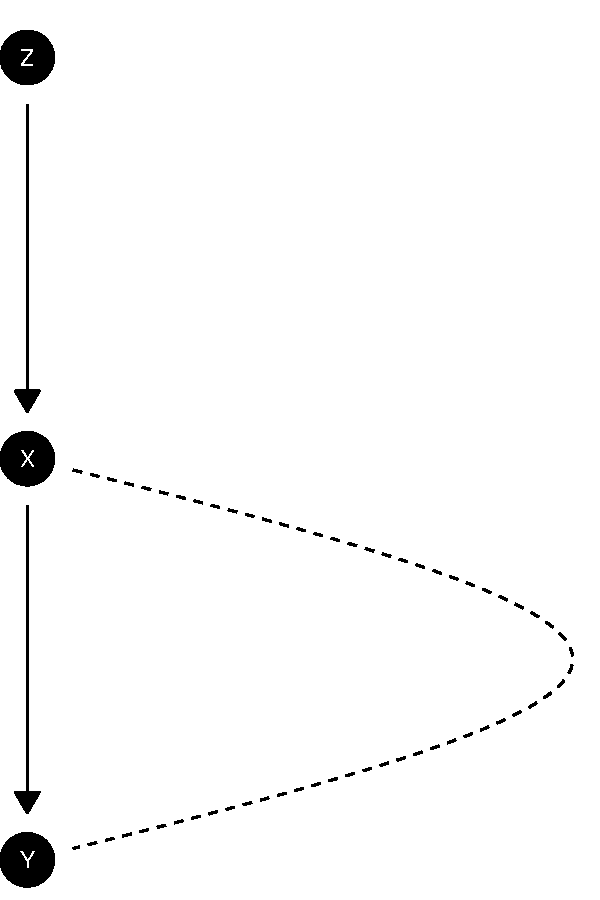
\includegraphics{paper_files/figure-pdf/fig-plots-1.pdf}

}

}

\subcaption{\label{fig-plots-1}Without options}
\end{minipage}%
%
\begin{minipage}[t]{0.50\linewidth}

{\centering 

\raisebox{-\height}{

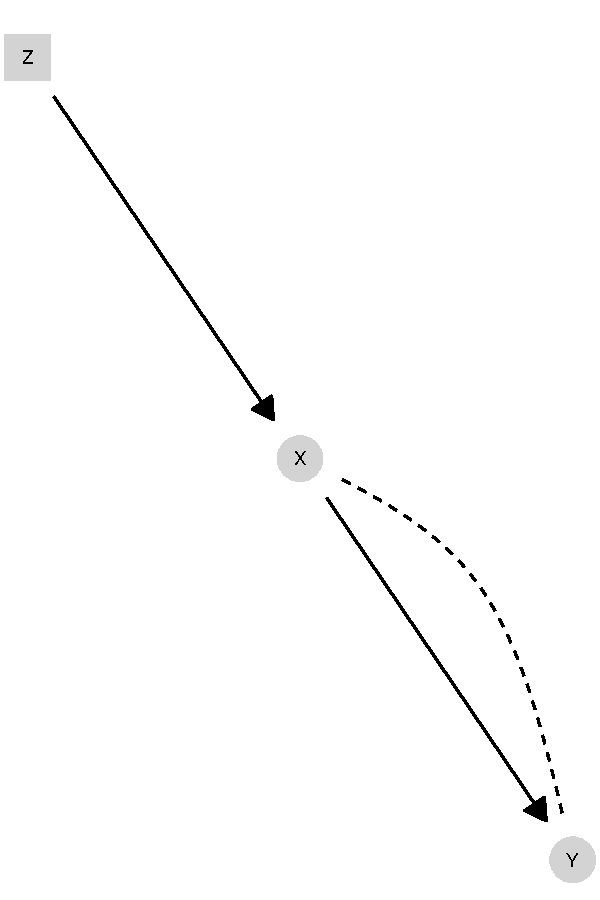
\includegraphics{paper_files/figure-pdf/fig-plots-2.pdf}

}

}

\subcaption{\label{fig-plots-2}With options}
\end{minipage}%

\caption{\label{fig-plots}Examples of model graphs.}

\end{figure}

\hypertarget{model-characterization}{%
\subsection{Model characterization}\label{model-characterization}}

When a model is defined, a set of objects is generated. These are the
key quantities that are used for all inference. Table~\ref{tbl-core}
summarizes the core components of a model, providing a brief explanation
for each one.

The first element is a \texttt{statement} which defines how the nodes in
the model are related, specified by the user using \texttt{dagitty}
syntax. The second element, \texttt{dag}, is a data frame that outlines
the parent-child relationships within the model. The element
\texttt{nodes} is simply a list of the names of the nodes in the model.
Lastly, \texttt{parents\_df,} is a table listing the nodes, indicating
if they are ``root'' nodes (nodes with no parents among the set of
specified nodes), and showing how many parents each node has.

The model includes additional elements, \texttt{nodal\_types,}
\texttt{parameters\_df,} and \texttt{causal\_types,} which we explain in
detail later.

\hypertarget{tbl-core}{}
\begin{longtable}[]{@{}
  >{\raggedright\arraybackslash}p{(\columnwidth - 2\tabcolsep) * \real{0.3000}}
  >{\raggedright\arraybackslash}p{(\columnwidth - 2\tabcolsep) * \real{0.7000}}@{}}
\caption{\label{tbl-core}Core Elements of a Causal
Model.}\tabularnewline
\toprule\noalign{}
\begin{minipage}[b]{\linewidth}\raggedright
Element
\end{minipage} & \begin{minipage}[b]{\linewidth}\raggedright
Description
\end{minipage} \\
\midrule\noalign{}
\endfirsthead
\toprule\noalign{}
\begin{minipage}[b]{\linewidth}\raggedright
Element
\end{minipage} & \begin{minipage}[b]{\linewidth}\raggedright
Description
\end{minipage} \\
\midrule\noalign{}
\endhead
\bottomrule\noalign{}
\endlastfoot
\texttt{statement} & A character string that describes directed causal
relations between variables in a causal model, where arrows denote that
one node is a potential cause of another. \\
\texttt{dag} & A data frame with columns `parent' and `children'
indicating how nodes relate to each other. \\
\texttt{nodes} & A list containing the nodes in the model. \\
\texttt{parents\_df} & A table listing nodes, whether they are root
nodes or not, and the number of parents they have. \\
\texttt{nodal\_types} & A list with the nodal types in the model. See
Section~\ref{sec-nodal-types} for more details. \\
\texttt{parameters\_df} & A data frame linking the model's parameters
with the nodal types of the model, as well as the family to which they
belong. See Section~\ref{sec-param-df} for more details. \\
\texttt{causal\_types} & A data frame listing causal types and the nodal
types that produce them. (See Causal Types Section) \\
\end{longtable}

After updating a model, two additional components are attached to it:

\begin{itemize}
\item
  A posterior distribution of the parameters in the model, generated by
  Stan. This distribution reflects the updated parameter values.
\item
  A list of other optional objects, \texttt{stan\_objects}. The
  \texttt{stan\_objects} can include the \texttt{stanfit} object and
  distributions over nodal types and event probabilities (\texttt{w}).
\end{itemize}

Table~\ref{tbl-additional} summarizes the objects attached to the model
after updating.

\hypertarget{tbl-additional}{}
\begin{longtable}[]{@{}
  >{\raggedright\arraybackslash}p{(\columnwidth - 2\tabcolsep) * \real{0.3000}}
  >{\raggedright\arraybackslash}p{(\columnwidth - 2\tabcolsep) * \real{0.7000}}@{}}
\caption{\label{tbl-additional}Additional Elements.}\tabularnewline
\toprule\noalign{}
\begin{minipage}[b]{\linewidth}\raggedright
Element
\end{minipage} & \begin{minipage}[b]{\linewidth}\raggedright
Description
\end{minipage} \\
\midrule\noalign{}
\endfirsthead
\toprule\noalign{}
\begin{minipage}[b]{\linewidth}\raggedright
Element
\end{minipage} & \begin{minipage}[b]{\linewidth}\raggedright
Description
\end{minipage} \\
\midrule\noalign{}
\endhead
\bottomrule\noalign{}
\endlastfoot
\texttt{posterior\_distribution} & The posterior distribution of the
updated parameters generated by Stan. \textbar{} \\
\texttt{stan\_objects} & A list of additional objects (see next
rows). \\
\texttt{data} & The data used for updating the model, always included in
\texttt{stan\_objects.} \\
\texttt{type\_distribution} & The updated distribution of the nodal
types, appended to \texttt{stan\_objects} by default. \\
\texttt{w} & A mapping from parameters to event probabilities,
optionally appended to \texttt{stan\_objects}. \\
\texttt{stan\_fit} & The \texttt{stanfit} object generated by Stan,
optionally appended to \texttt{stan\_objects}. \\
\end{longtable}

\hypertarget{sec-param-df}{%
\subsubsection{Parameters data frame}\label{sec-param-df}}

When a model is created, \texttt{CausalQueries} attaches a ``parameters
data frame'' which keeps track of model parameters, which belong
together in a family, and how they relate to causal types. This becomes
especially important for more complex models with confounding that might
involve more complicated mappings between parameters and nodal types. In
the case with no confounding the nodal types \emph{are} the parameters;
in cases with confounding there are generally more parameters than nodal
types.

We already saw a segment of a parameters data frame for a model with
confounding in Table~\ref{tbl-lipidspar}.

Table~\ref{tbl-params-df} shows the full parameters data frame for a
simple model, as generated by the following code:

\begin{verbatim}
R> make_model("X -> Y")$parameters_df
\end{verbatim}

\hypertarget{tbl-params-df}{}
\begin{table}[H]
\caption{\label{tbl-params-df}Example of Parameters Data Frame. }\tabularnewline

\centering
\resizebox{\linewidth}{!}{
\begin{tabular}{cccccccc}
\toprule
param\_names & node & gen & param\_set & nodal\_type & given & param\_value & priors\\
\midrule
X.0 & X & 1 & X & 0 &  & 0.50 & 1\\
X.1 & X & 1 & X & 1 &  & 0.50 & 1\\
Y.00 & Y & 2 & Y & 00 &  & 0.25 & 1\\
Y.10 & Y & 2 & Y & 10 &  & 0.25 & 1\\
Y.01 & Y & 2 & Y & 01 &  & 0.25 & 1\\
Y.11 & Y & 2 & Y & 11 &  & 0.25 & 1\\
\bottomrule
\end{tabular}}
\end{table}

here, as in Table~\ref{tbl-lipidspar}, each row in the data frame
corresponds to a single parameter.

The columns of the parameters data frame are understood as follows:

\begin{itemize}
\tightlist
\item
  \texttt{param\_names} gives the name of the parameter, in shorthand.
  For instance the parameter
  \(\lambda^X_0 = \Pr(\theta^X = \theta^X_0)\) has \texttt{par\_name}
  \texttt{X.0}.
\item
  \texttt{param\_value} gives the (possibly default) parameter values
  (probabilities).
\item
  \texttt{param\_set} indicates which parameters group together to form
  a simplex. The parameters in a set have parameter values that sum to
  1. In this example \(\lambda^X_0 + \lambda^X_1 = 1\).
\item
  \texttt{node} indicates the node associated with the parameter.
\item
  \texttt{nodal\_type} indicates the nodal types associated with the
  parameter.
\item
  \texttt{gen} indicates the place in the partial causal ordering
  (generation) of the node associated with the parameter
\item
  \texttt{priors} gives (possibly default) Dirichlet priors arguments
  for parameters in a set. Values of 1 (.5) for all parameters in a set
  implies uniform (Jeffrey's) priors over this set.
\end{itemize}

\hypertarget{sec-nodal-types}{%
\subsubsection{Nodal types}\label{sec-nodal-types}}

As described above, two units have the same \emph{nodal type} at node
\(Y\), \(\theta^Y\), if their outcome at \(Y\) responds in the same ways
to parents of \(Y\).

A binary node with \(k\) binary parents has \(2^{2^k}\) nodal types. The
reason is that with \(k\) parents, there are \(2^k\) possible values of
the parents and so \(2^{2^k}\) ways to respond to these possible
parental values. As a convention we say that a node with no parents has
two nodal types (0 or 1).

When a model is created the full set of nodal types is identified. These
are stored in the model. The labels for these nodal types indicate how
the unit responds to values of parents.

For instance, consider the model with two parents
\(X \rightarrow Y \leftarrow M.\) In such a case, the nodal types of
\(Y\) will have subscripts with four digits, with each digit
representing one of the possible combinations of values that \(Y\) can
take, given the values of its parents \(X\) and \(M.\) These
combinations include the value of \(Y\) when:

\begin{itemize}
\tightlist
\item
  \(X = 0\) and \(M = 0\),
\item
  \(X = 0\) and \(M = 1\),
\item
  \(X = 1\) and \(M = 0\),
\item
  \(X = 1\) and \(M = 1\).
\end{itemize}

As the number of parents increases, keeping track of what each digit
represents becomes more difficult. For instance, if \(Y\) had three
parents, its nodal types would have subscripts of eight digits, each
associated with the value that \(Y\) would take for each combination of
the three parents. The \texttt{interpret\_type()} function provides a
clear map to identify what each digit in the subscript represents. See
the examples below for models with two and three parents.

The \texttt{interpret\_type()} function can be called by the user to
obtain interpretations for the nodal types of each node in the model.

\begin{verbatim}
R> interpretations <- 
+  make_model("X -> Y <- M; W -> Y") |> 
+  interpret_type()
R> 
R> interpretations$Y
\end{verbatim}

\begin{verbatim}
#>   node position     display            interpretation
#> 1    Y        1 Y[*]******* Y | M = 0 & W = 0 & X = 0
#> 2    Y        2 Y*[*]****** Y | M = 1 & W = 0 & X = 0
#> 3    Y        3 Y**[*]***** Y | M = 0 & W = 1 & X = 0
#> 4    Y        4 Y***[*]**** Y | M = 1 & W = 1 & X = 0
#> 5    Y        5 Y****[*]*** Y | M = 0 & W = 0 & X = 1
#> 6    Y        6 Y*****[*]** Y | M = 1 & W = 0 & X = 1
#> 7    Y        7 Y******[*]* Y | M = 0 & W = 1 & X = 1
#> 8    Y        8 Y*******[*] Y | M = 1 & W = 1 & X = 1
\end{verbatim}

Interpretations are automatically provided as part of the model object.
A user can see them like this.

\begin{verbatim}
R> make_model("X -> Y")$nodal_types
\end{verbatim}

\hypertarget{causal-types}{%
\subsubsection{Causal types}\label{causal-types}}

Causal types are collections of nodal types. Two units are of the same
\emph{causal type} if they have the same nodal type at every node. For
example in a \(X \rightarrow M \rightarrow Y\) model,
\(\theta = (\theta^X_0, \theta^M_{01}, \theta^Y_{10})\) is a type that
has \(X=0\), \(M\) responds positively to \(X\), and \(Y\) responds
positively to \(M\).

When a model is created, the full set of causal types is identified.
These are stored in the model object:

\begin{verbatim}
R> lipids_model$causal_types |> head()
\end{verbatim}

\begin{verbatim}
#>            Z  X  Y
#> Z0.X00.Y00 0 00 00
#> Z1.X00.Y00 1 00 00
#> Z0.X10.Y00 0 10 00
#> Z1.X10.Y00 1 10 00
#> Z0.X01.Y00 0 01 00
#> Z1.X01.Y00 1 01 00
\end{verbatim}

In the lipids model there are \(2\times 4\times 4 = 32\) causal types. A
model with \(n_j\) nodal types at node \(j\) has \(\prod_jn_j\) causal
types. Thus the set of causal types can be large.

Knowledge of a causal type tells us what values a unit would take, on
all nodes, whether or not there are interventions. For example for a
model \(X \rightarrow M \rightarrow Y\) a type
\(\theta = (\theta^X_0, \theta^M_{01}, \theta^Y_{10})\) would imply data
\((X=0, M=0, Y=1)\) absent any intervention. (The converse of this, of
course, is the key to updating: observation of data \((X=0, M=0, Y=1)\)
result in more weight placed on \(\theta^X_0\), \(\theta^M_{01}\), and
\(\theta^Y_{10})\).) The general approach used by \texttt{CausalQueries}
for calculating outcomes from causal types is given in
Section~\ref{sec-propagation}.

\hypertarget{parameter-matrix}{%
\subsubsection{Parameter matrix}\label{parameter-matrix}}

The parameters data frame keeps track of parameter values and priors for
parameters but it does not provide a mapping between parameters and the
probability of causal types.

The parameter matrix---the ``\(P\) matrix''---can be added to the model
to provide this mapping. The \(P\) matrix has a row for each parameter
and a column for each causal type. For instance:

\begin{verbatim}
R> make_model("X -> Y") |> get_parameter_matrix()
\end{verbatim}

\begin{verbatim}
#> 
#> Rows are parameters, grouped in parameter sets
#> 
#> Columns are causal types
#> 
#> Cell entries indicate whether a parameter probability is used
#> in the calculation of causal type probability
#> 
#>      X0.Y00 X1.Y00 X0.Y10 X1.Y10 X0.Y01 X1.Y01 X0.Y11 X1.Y11
#> X.0       1      0      1      0      1      0      1      0
#> X.1       0      1      0      1      0      1      0      1
#> Y.00      1      1      0      0      0      0      0      0
#> Y.10      0      0      1      1      0      0      0      0
#> Y.01      0      0      0      0      1      1      0      0
#> Y.11      0      0      0      0      0      0      1      1
#> 
#>  
#>  param_set  (P)
#> 
\end{verbatim}

The probability of a causal type is given by the product of the
parameter values for parameters whose row in the \(P\) matrix contains a
1.

Later (e.g. Table~\ref{tbl-confound-params-mat}) we will see examples
where the \(P\) matrix helps keep track of parameters that are created
when confounding is added to a model.

The parameter matrix is generated on the fly as needed, but it can also
be added to the model using \texttt{set\_parameter\_matrix()}, which can
sometimes be useful to speed up operations:

\begin{verbatim}
R> model <- model |> set_parameter_matrix()
\end{verbatim}

\hypertarget{tailoring-models}{%
\subsection{Tailoring models}\label{tailoring-models}}

When a \texttt{dagitty} statement is provided to \texttt{make\_data()} a
model is formed with a set of default assumptions: in particular there
are no restrictions placed on nodal types and flat priors are assumed
over all parameters. These are features that can be adjusted after a
model is formed.

\hypertarget{restrictions}{%
\subsubsection{Setting restrictions}\label{restrictions}}

Sometimes for theoretical or practical reasons it is useful to constrain
the set of types. In \texttt{CausalQueries} this is done at the level of
nodal types, with restrictions on causal types following from
restrictions on nodal types.

To illustrate, in analyses of data with imperfect compliance, like we
saw in our motivating \texttt{lipids} model example, it is common to
impose a monotonicity assumption: that \(X\) does not respond negatively
to \(Z\). This is one of the conditions needed to interpret instrumental
variables estimates as (consistent) estimates of the complier average
treatment effect.

In \texttt{CausalQueries} we impose this assumption thus:

\begin{verbatim}
R> model_restricted <- 
+  make_model("Z -> X -> Y; X <-> Y")   |> 
+  set_restrictions("X[Z=1] < X[Z=0]")
\end{verbatim}

in words: we restrict by removing types for which \(X\) is decreasing in
\(Z\). If we wanted to retain only this nodal type, rather than remove
it, we could do so by stipulating \texttt{keep\ =\ FALSE}.

\begin{table}

\end{table}

We can use \texttt{get\_parameter\_matrix(model)} to view the resulting
parameter matrix in which both the set of parameters and the set of
causal types are restricted.

Setting restrictions sometimes involves using causal syntax; see
Section~\ref{sec-syntax} for a guide the syntax used by
\texttt{CausalQueries}.

Note:

\begin{itemize}
\tightlist
\item
  Restrictions have to operate on nodal types: restrictions on
  \emph{levels} of endogenous nodes are not allowed. This, for example,
  will fail:
  \texttt{make\_model("X\ -\textgreater{}\ Y")\ \textbar{}\textgreater{}\ set\_restrictions(statement\ =\ \ "(Y\ ==\ 1)")}.
  The reason is that it requests a correlated restriction on nodal types
  for \texttt{X} and \texttt{Y} which involves undeclared confounding.
\item
  Restrictions implicitly assume fixed values for \emph{all} parents of
  a node. For instance:
  \texttt{make\_model("A\ -\textgreater{}\ B\ \textless{}-\ C")\ \textbar{}\textgreater{}\ set\_restrictions("(B{[}C=1{]}==1)")}
  is interpreted as shorthand for the restriction
  \texttt{"B{[}C\ =\ 1,\ A\ =\ 0{]}==1\ \textbar{}\ B{[}C\ =\ 1,\ A\ =\ 1{]}==1"}.
  The \texttt{join\_by} argument can be used to indicate ``and'' rather
  than ``or'' relations on omitted parents.
\item
  To place restrictions on multiple nodes at the same time, provide
  these as a vector of restrictions. This is not permitted:
  \texttt{set\_restrictions("Y{[}X=1{]}==1\ \&\ X==1")}, since it
  requests correlated restrictions. This however is allowed:
  \texttt{set\_restrictions(c("Y{[}X=1{]}==1",\ "X==1"))}.
\item
  Use the \texttt{keep} argument to indicate whether nodal types should
  be dropped (default) or retained.
\item
  Restrictions based on causal statements can use helpers,
  \texttt{decreasing()}, \texttt{increasing()}, \texttt{complements()}
  and similar. For instance
  \texttt{set\_restrictions(decreasing("X",\ "Y"))}
\item
  Restrictions can be set using nodal type labels.
\end{itemize}

\begin{verbatim}
R> make_model("S -> C -> Y <- R <- X; X -> C -> R") |>
+  set_restrictions(labels = list(C = "1000", R = "0001", Y = "0001"), 
+                   keep = TRUE)
\end{verbatim}

\begin{itemize}
\tightlist
\item
  Wild cards can be used in nodal type labels:
\end{itemize}

\begin{verbatim}
R> make_model("X -> Y") |>
+  set_restrictions(labels = list(Y = "?0"))
\end{verbatim}

\begin{itemize}
\tightlist
\item
  in models with confounding restrictions can be added to nodal types
  conditional on the values of other nodal types; this is done using a
  ``given'' argument.
\end{itemize}

\begin{verbatim}
R> model <- make_model("X -> Y -> Z; X <-> Z") %>%
+ set_restrictions(labels = list(X = '0', Y = c('00', '11'), Z = '00'), 
+                  given = c(NA, NA, 'X.1')) |>
+  get_parameter_matrix() 
\end{verbatim}

\hypertarget{tbl-confound-params-mat}{}
\begin{table}
\caption{\label{tbl-confound-params-mat}Restrictions on models with confounds. }\tabularnewline

\centering
\begin{tabular}{lcccccc}
\toprule
  & X1.Y10.Z10 & X1.Y01.Z10 & X1.Y10.Z01 & X1.Y01.Z01 & X1.Y10.Z11 & X1.Y01.Z11\\
\midrule
X.1 & 1 & 1 & 1 & 1 & 1 & 1\\
Y.10 & 1 & 0 & 1 & 0 & 1 & 0\\
Y.01 & 0 & 1 & 0 & 1 & 0 & 1\\
Z.10\_X.1 & 1 & 1 & 0 & 0 & 0 & 0\\
Z.01\_X.1 & 0 & 0 & 1 & 1 & 0 & 0\\
Z.11\_X.1 & 0 & 0 & 0 & 0 & 1 & 1\\
\bottomrule
\end{tabular}
\end{table}

\hypertarget{sec-confounding}{%
\subsubsection{Allowing confounding}\label{sec-confounding}}

Unobserved confounding between two (or more) nodes arises when the nodal
types for the nodes are not independent.

In the \(X \rightarrow Y\) graph, for instance, there are 2 nodal types
for \(X\) and 4 for \(Y\). There are thus 8 joint nodal types (or causal
types), as shown in Table~\ref{tbl-joint}.

\hypertarget{tbl-joint}{}
\begin{longtable}[]{@{}
  >{\centering\arraybackslash}p{(\columnwidth - 6\tabcolsep) * \real{0.2500}}
  >{\centering\arraybackslash}p{(\columnwidth - 6\tabcolsep) * \real{0.2500}}
  >{\centering\arraybackslash}p{(\columnwidth - 6\tabcolsep) * \real{0.2500}}
  >{\centering\arraybackslash}p{(\columnwidth - 6\tabcolsep) * \real{0.2500}}@{}}
\caption{\label{tbl-joint}Nodal Types in \(X \rightarrow Y\)
Model.}\tabularnewline
\toprule\noalign{}
\begin{minipage}[b]{\linewidth}\centering
\(\theta^Y\) \textbf{\textbackslash{}} \(\theta^X\)
\end{minipage} & \begin{minipage}[b]{\linewidth}\centering
\textbf{0}
\end{minipage} & \begin{minipage}[b]{\linewidth}\centering
\textbf{1}
\end{minipage} & \begin{minipage}[b]{\linewidth}\centering
\(\sum\)
\end{minipage} \\
\midrule\noalign{}
\endfirsthead
\toprule\noalign{}
\begin{minipage}[b]{\linewidth}\centering
\(\theta^Y\) \textbf{\textbackslash{}} \(\theta^X\)
\end{minipage} & \begin{minipage}[b]{\linewidth}\centering
\textbf{0}
\end{minipage} & \begin{minipage}[b]{\linewidth}\centering
\textbf{1}
\end{minipage} & \begin{minipage}[b]{\linewidth}\centering
\(\sum\)
\end{minipage} \\
\midrule\noalign{}
\endhead
\bottomrule\noalign{}
\endlastfoot
\textbf{00} & \(\Pr(\theta^X_0, \theta^Y_{00})\) &
\(\Pr(\theta^X_1, \theta^Y_{00})\) & \(\Pr(\theta^Y_{00})\) \\
\textbf{10} & \(\Pr(\theta^X_0, \theta^Y_{10})\) &
\(\Pr(\theta^X_1, \theta^Y_{10})\) & \(\Pr(\theta^Y_{10})\) \\
\textbf{01} & \(\Pr(\theta^X_0, \theta^Y_{01})\) &
\(\Pr(\theta^X_1, \theta^Y_{01})\) & \(\Pr(\theta^Y_{01})\) \\
\textbf{11} & \(\Pr(\theta^X_0, \theta^Y_{11})\) &
\(\Pr(\theta^X_1, \theta^Y_{11})\) & \(\Pr(\theta^Y_{11})\) \\
\(\sum\) & \(\Pr(\theta^X_0)\) & \(\Pr(\theta^X_1)\) & 1 \\
\end{longtable}

Table~\ref{tbl-joint} has eight interior elements and so an
unconstrained joint distribution would have \(7\) degrees of freedom. A
no confounding assumption means that
\(\Pr(\theta^X | \theta^Y) = \Pr(\theta^X)\), or
\(\Pr(\theta^X, \theta^Y) = \Pr(\theta^X)\Pr(\theta^Y)\). In this case
we just put a distribution on the marginals and there would be \(3\)
degrees of freedom for \(Y\) and \(1\) for \(X\), totaling \(4\) rather
than \(7\).

\begin{verbatim}
R> confounded <- make_model("X -> Y ; X <-> Y")
\end{verbatim}

\hypertarget{tbl-confound-params-df}{}
\begin{table}[H]
\caption{\label{tbl-confound-params-df}Parameters Data Frame for Model with Confounding. }\tabularnewline

\centering
\resizebox{\linewidth}{!}{
\begin{tabular}{cccccccc}
\toprule
param\_names & node & gen & param\_set & nodal\_type & given & param\_value & priors\\
\midrule
X.0 & X & 1 & X & 0 &  & 0.50 & 1\\
X.1 & X & 1 & X & 1 &  & 0.50 & 1\\
Y.00\_X.0 & Y & 2 & Y.X.0 & 00 & X.0 & 0.25 & 1\\
Y.10\_X.0 & Y & 2 & Y.X.0 & 10 & X.0 & 0.25 & 1\\
Y.01\_X.0 & Y & 2 & Y.X.0 & 01 & X.0 & 0.25 & 1\\
Y.11\_X.0 & Y & 2 & Y.X.0 & 11 & X.0 & 0.25 & 1\\
Y.00\_X.1 & Y & 2 & Y.X.1 & 00 & X.1 & 0.25 & 1\\
Y.10\_X.1 & Y & 2 & Y.X.1 & 10 & X.1 & 0.25 & 1\\
Y.01\_X.1 & Y & 2 & Y.X.1 & 01 & X.1 & 0.25 & 1\\
Y.11\_X.1 & Y & 2 & Y.X.1 & 11 & X.1 & 0.25 & 1\\
\bottomrule
\end{tabular}}
\end{table}

The parameters data frame for this model would have two parameter
families for parameters associated with the node \(Y\). Each family
captures the conditional distribution of \(Y\)'s nodal types, given
\(X\). For instance the parameter \texttt{Y01\_X.1} can be interpreted
as \(\Pr(\theta^Y = \theta^Y_{01} | X=1)\). See again
Table~\ref{tbl-lipidspar} for an example of a parameters matrix with
confounding.

To see exactly how the parameters map to causal types we can view the
parameter matrix thus:

\begin{verbatim}
R> get_parameter_matrix(confounded)
\end{verbatim}

\hypertarget{tbl-confound-param-matrix}{}
\begin{table}
\caption{\label{tbl-confound-param-matrix}Parameter Matrix for Model with Confounding. }\tabularnewline

\centering
\resizebox{\linewidth}{!}{
\begin{tabular}{lcccccccc}
\toprule
  & X0.Y00 & X1.Y00 & X0.Y10 & X1.Y10 & X0.Y01 & X1.Y01 & X0.Y11 & X1.Y11\\
\midrule
X.0 & 1 & 0 & 1 & 0 & 1 & 0 & 1 & 0\\
X.1 & 0 & 1 & 0 & 1 & 0 & 1 & 0 & 1\\
Y.00\_X.0 & 1 & 0 & 0 & 0 & 0 & 0 & 0 & 0\\
Y.10\_X.0 & 0 & 0 & 1 & 0 & 0 & 0 & 0 & 0\\
Y.01\_X.0 & 0 & 0 & 0 & 0 & 1 & 0 & 0 & 0\\
Y.11\_X.0 & 0 & 0 & 0 & 0 & 0 & 0 & 1 & 0\\
Y.00\_X.1 & 0 & 1 & 0 & 0 & 0 & 0 & 0 & 0\\
Y.10\_X.1 & 0 & 0 & 0 & 1 & 0 & 0 & 0 & 0\\
Y.01\_X.1 & 0 & 0 & 0 & 0 & 0 & 1 & 0 & 0\\
Y.11\_X.1 & 0 & 0 & 0 & 0 & 0 & 0 & 0 & 1\\
\bottomrule
\end{tabular}}
\end{table}

The output is shown in Table~\ref{tbl-confound-param-matrix}.
Importantly, the \(P\) matrix works as before, despite confounding. We
can assess the probability of causal types by multiplying the
probabilities of the constituent parameters.

Table~\ref{tbl-dof} illustrates more generally how the number of
independent parameters depends on the nature of possible confounding.

\hypertarget{tbl-dof}{}
\begin{table}
\caption{\label{tbl-dof}Number of different independent parameters (degrees of freedom) for
different 3 node models. }\tabularnewline

\centering
\begin{tabular}{lc}
\toprule
Model & dof\\
\midrule
X -> Y <- W & 17\\
X -> Y <- W; X <-> W & 18\\
X -> Y <- W; X <-> Y; W <-> Y & 62\\
X -> Y <- W; X <-> Y; W <-> Y; X <->W & 63\\
X -> W -> Y <- X & 19\\
X -> W -> Y <- X; W <-> Y & 64\\
X -> W -> Y <- X; X <-> W; W <-> Y & 127\\
X -> W -> Y <- X; X <-> W; W <-> Y; X <-> Y & 127\\
\bottomrule
\end{tabular}
\end{table}

\hypertarget{priors}{%
\subsubsection{Setting Priors}\label{priors}}

Priors on model parameters can be added to the parameters data frame.
The priors are interpreted as ``alpha'' arguments for a Dirichlet
distribution. The Dirichlet distribution is a probability distribution
over an \(n-1\) dimensional unit simplex. It can be thought of as a
generalization of the Beta distribution and is parameterized by an
\(n\)-dimensional positive vector \(\alpha\). Thus for example a
Dirichlet with \(\alpha = (1, 1, 1, 1, 1)\) gives a probability
distribution over all non negative \(5\)-dimensional vectors that sum to
\(1\), e.g.~\((0.1, 0.1, 0.1, 0.1, 0.6)\) or
\((0.1, 0.2, 0.3, 0.3, 0.1)\). This particular value for \(\alpha\)
implies that all such vectors are equally likely. Other values for
\(\alpha\) can be used to control the expectation for each dimension as
well as certainty. Thus for instance the vector
\(\alpha = (100, 1, 1, 1, 100)\) would result in more weight on
distributions that are close to \((0.5, 0, 0, 0, 0.5)\).

In \texttt{CausalQueries}, priors are generally specified over the
distribution of nodal types (or over the conditional distribution of
nodal types, when there is confounding). Thus for instance in an
\(X \rightarrow Y\) model we have one Dirichlet distribution over the
two types for \(\theta^X\) and one Dirichlet distribution over the four
types for \(\theta^Y\).

By default, priors are set to unity, corresponding to uniform priors. To
retrieve the model's priors we can run the following code:

\begin{verbatim}
R> make_model("X -> Y") |> get_priors()
\end{verbatim}

\begin{verbatim}
#>  X.0  X.1 Y.00 Y.10 Y.01 Y.11 
#>    1    1    1    1    1    1
\end{verbatim}

Alternatively you could set Jeffreys priors using \texttt{set\_priors}
as follows:

\begin{verbatim}
R> make_model("X -> Y") |> 
+  set_priors(distribution = "jeffreys") 
\end{verbatim}

You can also add custom priors. Custom priors are most simply specified
by being added as a vector of numbers using \texttt{set\_priors}. For
instance:

\begin{verbatim}
R> make_model("X -> Y") |> 
+  set_priors(1:6) |> 
+  get_priors()
\end{verbatim}

\begin{verbatim}
#>  X.0  X.1 Y.00 Y.10 Y.01 Y.11 
#>    1    2    3    4    5    6
\end{verbatim}

The priors here should be interpreted as indicating:

\begin{itemize}
\tightlist
\item
  \(\alpha_X = (1,2)\), which implies a distribution over
  \((\lambda^X_0, \lambda^X_1)\) centered on \((1/3, 2/3)\).
\item
  \(\alpha_Y = (3,4,5,6)\), which implies a distribution over
  \((\lambda^Y_{00}, \lambda^Y_{10}, \lambda^Y_{01} \lambda^Y_{11})\)
  centered on \((3/18, 4/18, 5/18, 6/18)\).
\end{itemize}

For larger models it can be hard to provide priors as a vector of
numbers. For that reason \texttt{set\_priors} allows for more targeted
modifications of the parameter vector. For instance:

\begin{verbatim}
R> make_model("X -> Y") |>
+  set_priors(statement = "Y[X=1] > Y[X=0]", alphas = 3) |>
+  get_priors()
\end{verbatim}

\begin{verbatim}
#>  X.0  X.1 Y.00 Y.10 Y.01 Y.11 
#>    1    1    1    1    3    1
\end{verbatim}

As setting priors simply requires mapping alpha values to parameters,
the process reduces to selecting rows of the \texttt{parmeters\_df} data
frame, at which to alter values. When specifying a causal statement as
above, \texttt{CausalQueries} internally identifies nodal types that are
consistent with the statement, which in turn identify parameters to
alter priors for.

We can achieve the same result as above by specifying nodal types for
which we would like to adjust the priors:

\begin{verbatim}
R> make_model("X -> Y") |>
+  set_priors(nodal_type = "01", alphas = 3) |>
+  get_priors()
\end{verbatim}

\begin{verbatim}
#>  X.0  X.1 Y.00 Y.10 Y.01 Y.11 
#>    1    1    1    1    3    1
\end{verbatim}

or even parameter names

\begin{verbatim}
R> make_model("X -> Y") |>
+  set_priors(param_names = "Y.01", alphas = 3) |>
+  get_priors()
\end{verbatim}

\begin{verbatim}
#>  X.0  X.1 Y.00 Y.10 Y.01 Y.11 
#>    1    1    1    1    3    1
\end{verbatim}

Indeed \texttt{set\_priors()} allows for the specification of any
non-redundant combination of arguments on the \texttt{param\_names},
\texttt{node}, \texttt{nodal\_type}, \texttt{param\_set} and
\texttt{given} columns of \texttt{parameters\_df} to uniquely identify
parameters to set priors for. Alternatively a fully formed subsetting
statement may be supplied to \texttt{alter\_at}. Since all these
arguments get mapped to the parameters they identify internally they may
be used interchangeably.\footnote{See \texttt{?set\_priors} and
  \texttt{?make\_priors} for many more examples.}

Thus the following two specifications of priors are equivalent:

\begin{verbatim}
R> model <- make_model("X -> M -> Y; X <-> Y")
R> 
R> model |>
+  set_priors(node = "Y", 
+             nodal_type = c("01","11"), 
+             given = "X.1", 
+             alphas = c(3,2)) 
R> 
R> model |>
+  set_priors(
+    alter_at = 
+      "node == 'Y' & nodal_type %in% c('01','11') & given == 'X.1'", 
+    alphas = c(3,2)) 
\end{verbatim}

It should be noted that while highly targeted prior setting is
convenient and flexible; it should be done with caution. Setting priors
on specific parameters in complex models; especially models involving
confounding, may strongly affect inferences in intractable ways.

We additionally note that flat priors over nodal types do not
necessarily translate into flat priors over queries. ``Flat'' priors
over parameters in a parameter family put equal weight on each nodal
type, but this in turn can translate into strong assumptions on causal
quantities of interest.

For instance in an \(X \rightarrow Y\) model in which negative effects
are ruled out, the average causal effect implied by ``flat'' priors is
\(1/3\). This can be seen by querying the model as follows:

\begin{verbatim}
R> make_model("X -> Y") |>
+  set_restrictions(decreasing("X", "Y")) |>
+  query_model("Y[X=1] - Y[X=0]", using = "priors")
\end{verbatim}

More subtly the \emph{structure} of a model, coupled with flat priors,
has substantive importance for priors on causal quantities. For instance
with flat priors, priors on the probability that \(X\) has a positive
effect on \(Y\) in the model \(X \rightarrow Y\) is centered on \(1/4\).
But priors on the probability that \(X\) has a positive effect on \(Y\)
in the model \(X \rightarrow M \rightarrow Y\) is centered on \(1/8\).

Again, you can use \texttt{query\_model} to figure out what flat (or
other) priors over parameters imply for priors over causal quantities:

\begin{verbatim}
R> make_model("X -> Y") |>
+  query_model("Y[X=1] > Y[X=0]", using = "priors")
R> 
R> make_model("X -> M -> Y") |>
+  query_model("Y[X=1] > Y[X=0]", using = "priors")
\end{verbatim}

Caution regarding priors is particularly important when models are not
identified, as is the case for many of the models considered here. In
such cases, for some quantities, the marginal posterior distribution
simply reflects the marginal prior distribution
\citep{poirier_revising_1998}.

The key point here is to make sure you do not fall into a trap of
thinking that ``uninformative'' priors make no commitments regarding the
values of causal quantities of interest. They do, and the implications
of flat priors for causal quantities can depend on the structure of the
model. Moreover for some inferences from causal models the priors can
matter a lot even if you have a lot of data. In such cases it can be
helpful to know what priors on parameters imply for priors on causal
quantities of interest (by using \texttt{query\_model()}) and to assess
how much conclusions depend on priors (by comparing results across
models that vary in their priors).

\hypertarget{parameters}{%
\subsubsection{Setting Parameters}\label{parameters}}

By default, models have a vector of parameter values included in the
\texttt{parameters\_df} data frame. These are useful for generating
data, or for situations, such as process tracing, when one wants to make
inferences about causal types (\(\theta\)), given case level data, under
the assumption that the model is known.

The logic for setting parameters is similar to that for setting priors:
effectively we need to place values on the probability of nodal types.
The key difference is that whereas the \(\alpha\) value placed on a
nodal types can be any positive number---capturing our certainty over
the parameter value---the parameter values must lie in the unit
interval, \([0,1]\). In general if parameter values are passed that do
not lie in the unit interval, these are normalized so that they do.

Consider the causal model below. It has two parameter sets, one for
\(X\) and one for \(Y\), with six nodal types, two corresponding to
\(X\) and four corresponding to \(Y\). The key feature of the parameters
is that they must sum to 1 within each parameter set.

\begin{verbatim}
R> make_model("X -> Y") |> 
+  get_parameters()
\end{verbatim}

\begin{verbatim}
#>  X.0  X.1 Y.00 Y.10 Y.01 Y.11 
#> 0.50 0.50 0.25 0.25 0.25 0.25
\end{verbatim}

The example below illustrates a change in the value of the parameter
\(Y\) in the case it is increasing in \(X\). Here nodal type
\texttt{Y.Y01} is set to be 0.5, while the other nodal types of this
parameter set were renormalized so that the parameters in the set still
sum to one.

\begin{verbatim}
R> make_model("X -> Y") |>
+  set_parameters(statement = "Y[X=1] > Y[X=0]", parameters = .5) |>
+  get_parameters()
\end{verbatim}

\begin{verbatim}
#>       X.0       X.1      Y.00      Y.10      Y.01      Y.11 
#> 0.5000000 0.5000000 0.1666667 0.1666667 0.5000000 0.1666667
\end{verbatim}

\hypertarget{drawing-and-manipulating-data}{%
\subsection{Drawing and manipulating
data}\label{drawing-and-manipulating-data}}

Once a model has been defined it is possible to simulate data from the
model using the \texttt{make\_data} function. This can be useful for
instance for assessing the expected performance of a model given data
drawn from some speculated set of parameter values.

\begin{verbatim}
R> model <- make_model("X -> M -> Y") 
\end{verbatim}

\hypertarget{drawing-data-basics}{%
\subsubsection{Drawing data basics}\label{drawing-data-basics}}

By default, the parameters used are taken from
\texttt{model\$parameters\_df}.

\begin{verbatim}
R> sample_data_1 <- 
+  model |> 
+  make_data(n = 4)
\end{verbatim}

However you can also specify parameters directly or use parameter draws
from a prior or posterior distribution. For instance:

\begin{verbatim}
R> make_data(model, n = 3, param_type = "prior_draw")
\end{verbatim}

\begin{verbatim}
#>   X M Y
#> 1 0 0 1
#> 2 0 0 1
#> 3 1 0 0
\end{verbatim}

Note that the data is returned ordered by data type as in the example
above.

\hypertarget{drawing-incomplete-data}{%
\subsubsection{Drawing incomplete data}\label{drawing-incomplete-data}}

\texttt{CausalQueries} can be used in settings in which researchers have
gathered different amounts of data for different nodes. For instance
gathering \(X\) and \(Y\) data for all units but \(M\) data only for
some.

The function \texttt{make\_data} allows you to draw data like this if
you specify a data strategy indicating the probabilities of observing
data on different nodes, possibly as a function of prior nodes observed.

\begin{verbatim}
R> set.seed(1)
R> 
R> sample_data_2 <-
+  make_data(model,
+            n = 8,
+            nodes = list(c("X", "Y"), "M"),
+            probs = list(1, .5),
+            subsets = list(TRUE, "X==1 & Y==0"))
\end{verbatim}

\begin{verbatim}
#> # A tibble: 2 x 5
#>   node_names nodes     n_steps probs subsets    
#>   <chr>      <list>    <lgl>   <dbl> <chr>      
#> 1 X, Y       <chr [2]> NA        1   TRUE       
#> 2 M          <chr [1]> NA        0.5 X==1 & Y==0
\end{verbatim}

\begin{verbatim}
R> sample_data_2
\end{verbatim}

\begin{verbatim}
#>   X  M Y
#> 1 0 NA 0
#> 2 0 NA 1
#> 3 1 NA 0
#> 4 1 NA 1
#> 5 1 NA 1
#> 6 1  1 0
#> 7 1 NA 0
#> 8 1  1 0
\end{verbatim}

\hypertarget{reshaping-data}{%
\subsubsection{Reshaping data}\label{reshaping-data}}

Whereas data naturally comes in long form, with a row per observation,
as in the examples above, the data passed to Stan is in a compact form,
which records only the number of units of each data type, grouped by
data ``strategy''---an indicator of the nodes for which data was
gathered. \texttt{CausalQueries} includes functions that lets you move
between these two forms in case of need.

\begin{verbatim}
R> sample_data_2 |> collapse_data(model)
\end{verbatim}

\begin{verbatim}
#>     event strategy count
#> 1  X0M0Y0      XMY     0
#> 2  X1M0Y0      XMY     0
#> 3  X0M1Y0      XMY     0
#> 4  X1M1Y0      XMY     2
#> 5  X0M0Y1      XMY     0
#> 6  X1M0Y1      XMY     0
#> 7  X0M1Y1      XMY     0
#> 8  X1M1Y1      XMY     0
#> 9    X0Y0       XY     1
#> 10   X1Y0       XY     2
#> 11   X0Y1       XY     1
#> 12   X1Y1       XY     2
\end{verbatim}

In the same way it is possible to move from ``compact data'' to ``long
data'' using \texttt{expand\_data()}. Note that \texttt{NA}'s are
interpreted as data not having been sought. So in the case of
\texttt{sample\_data\_2} the interpretation is that there are two data
strategies: data on \(Y\), \(M\) and \(X\) was sought in two cases only;
data on \(Y\) and \(X\) only was sought in six cases.

\hypertarget{sec-update}{%
\section{Updating models}\label{sec-update}}

The approach used by the \texttt{CausalQueries} package to updating
parameter values given observed data uses Stan
\citep{carpenter_stan_2017}.

Below we explain the data required by the generic Stan program
implemented in the package, the structure of that program, and then show
how to use the package to produce posterior draws of parameters.

\hypertarget{data-for-stan}{%
\subsection{Data for Stan}\label{data-for-stan}}

We use a generic Stan program that works for all binary causal models.
The main advantage of the generic program we implement is that it allows
us to pass the details of causal model as data inputs to Stan instead of
generating individual Stan program for each causal model.

The data required by the Stan program includes vectors of observed data
(\texttt{Y}) and priors on parameters (\texttt{lambdas\_prior}) as well
as a set of matrices required for the mapping between events, data
types, causal types and parameters. The latter includes:

\begin{itemize}
\tightlist
\item
  A parameter matrix (\texttt{P}) that tells Stan how many parameters
  there are, and how they map into causal types,
\item
  A matrix that maps parameters to data types (\texttt{parmap}), and
\item
  An event matrix (\texttt{E}) that relates data types into patterns of
  observed data (events) in cases where there are incomplete
  observations.
\end{itemize}

In addition data includes counts of all relevant quantities as well as
start and end positions of parameters pertaining to specific nodes and
of distinct data strategies.

The internal function \texttt{prep\_stan\_data()} takes model and data
as arguments and produces a list with all objects described above that
are required by the generic Stan program. Generally, package users do
not need to call the \texttt{prep\_stan\_data()} function directly to
update the model. If further inspection of the data required by the Stan
program is required, you can do so using the code below

\begin{verbatim}
R> sample_data_2 |> 
+  collapse_data(model = model) |> 
+  CausalQueries:::prep_stan_data(model = model)
\end{verbatim}

\hypertarget{how-the-stan-program-works}{%
\subsection{How the Stan program
works}\label{how-the-stan-program-works}}

The Stan model involves the following elements:

\begin{itemize}
\tightlist
\item
  A specification of priors over sets of parameters
\item
  A mapping from parameters to event probabilities, \(w\)
\item
  A likelihood function.
\end{itemize}

\hypertarget{probability-distributions-over-parameter-sets}{%
\subsubsection{Probability distributions over parameter
sets}\label{probability-distributions-over-parameter-sets}}

We are interested in ``sets'' of parameters. In the case without
confounding these sets correspond to the nodal types for each node: we
have a probability distribution over the set of nodal types. In cases
with confounding these are sets of nodal types for a give node
\emph{given} values of other nodes: we have characterize the probability
of each nodal type in a set given the values of nodal types for other
nodes.

We express priors over these parameter sets using multiple Dirichlet
distributions. In practice because we are dealing with multiple
simplices of varying length, it is easier to express priors over gamma
distributions with a unit scale parameter and shape parameter
corresponding to the Dirichlet priors, \(\alpha\). We make use of the
fact that \(\lambda^X_0 \sim Gamma(\alpha^X_0,1)\) and
\(\lambda^X_1 \sim Gamma(\alpha^X_1,1)\) then
\(\frac{1}{\lambda^X_0 +\lambda^X_1}(\lambda^X_0, \lambda^X_1) \sim Dirichlet(\alpha^X_0, \alpha^X_1)\)\footnote{For
  a discussion of implementation of this approach in Stan see discussion
  (here){[}https://discourse.mc-stan.org/t/ragged-array-of-simplexes/1382{]}.}

To illustrate, in the \(X \rightarrow Y\) model we have two parameter
sets (\texttt{param\_sets}). The first is
\(\lambda^X \in \{\lambda^X_0, \lambda^X_1\}\) whose elements give the
probability that \(X\) is 0 or 1. These two probabilities sum to one.
The second parameter set is
\(\lambda^Y \in \{\lambda^Y_{00}, \lambda^Y_{10}, \lambda^Y_{01} \lambda^Y_{11}\}\).
These are also probabilities and their values sum to one. Note in all
that we have 6 parameters but just 1 + 3 = 4 degrees of freedom. We have
a 2 dimensional Dirichlet distribution over the \(X\) nodal types
(equivalently, a Beta distribution) and a 4 dimensional Dirichlet over
the \(Y\) nodal types.

\hypertarget{event-probabilities}{%
\subsubsection{Event probabilities}\label{event-probabilities}}

For any candidate parameter vector \(\lambda\) we calculate the
probability of \emph{data} types. This is done using a matrix that maps
from parameters into data types, \texttt{parmap}. In cases without
confounding there is a column for each data type; the matrix indicates
which nodes in each set ``contribute'' to the data type, and the
probability of the data type is found by summing within sets and taking
the product over sets.

The following code:

\begin{verbatim}
R> make_model("X -> Y") |> 
+  get_parmap() 
\end{verbatim}

\hypertarget{tbl-parmap}{}
\begin{table}
\caption{\label{tbl-parmap}Mapping from parameters to data types. }\tabularnewline

\centering
\begin{tabular}{lcccc}
\toprule
  & X0Y0 & X1Y0 & X0Y1 & X1Y1\\
\midrule
X.0 & 1 & 0 & 1 & 0\\
X.1 & 0 & 1 & 0 & 1\\
Y.00 & 1 & 1 & 0 & 0\\
Y.10 & 0 & 1 & 1 & 0\\
Y.01 & 1 & 0 & 0 & 1\\
Y.11 & 0 & 0 & 1 & 1\\
\bottomrule
\end{tabular}
\end{table}

yields Table~\ref{tbl-parmap}, which can be used to calculate event
probabilities. For instance the probability of data type \texttt{X0Y0},
\(w_{00}\) is
\(\lambda^X_0\times \lambda^Y_{00} + \lambda^X_0\times \lambda^Y_{01}\).
This is found by combining a parameter vector with the first column of
\texttt{parmap}, taking the product of the probability of \texttt{X.0}
and the \emph{sum} of the probabilities for \texttt{Y.00} and
\texttt{Y.01}.

In cases with confounding the approach is similar except that the
\texttt{parmap} matrix can contain multiple columns for each data type
to capture non-independence between nodes.

In the case of incomplete data we first identify the set of ``data
strategies'', where a collection of a data strategy might be of the form
``gather data on \(X\) and \(M\), but not \(Y\), for \(n_1\) cases and
gather data on \(X\) and \(Y\), but not \(M\), for \(n_2\) cases. The
probability of an observed event, within a data strategy, is given by
summing the probabilities of the types that could give rise to the
incomplete data. For example \(X\) is observed, but \(Y\) is not, then
the probability of \(X=0, Y = \text{NA}\) is \(w_{00} +w_{01}\). The
matrix \(E\) is passed to Stan to figure out which event probabilities
need to be combined for events with missing data.

\hypertarget{data-probability}{%
\subsubsection{Data probability}\label{data-probability}}

Once we have the event probabilities in hand for each data strategy we
are ready to calculate the probability of the data. For a given data
strategy this is given by a multinomial distribution with these event
probabilities. When there is incomplete data, and so multiple data
strategies, this is given by the the product of the multinomial
probabilities for each strategy.

\hypertarget{implementation}{%
\subsection{Implementation}\label{implementation}}

To update a \texttt{CausalQueries} model with data use:

\begin{verbatim}
R> update_model(model, data)
\end{verbatim}

where the data argument is a dataset containing some or all of the nodes
in the model. \texttt{update\_model()} relies on
\texttt{rstan::sampling()} to draw from posterior distribution and one
can pass any additional arguments accepted by \texttt{rstan::sampling()}
in \texttt{...}.

\hypertarget{parallelization}{%
\subsection{Parallelization}\label{parallelization}}

If you have multiple cores you can do parallel processing by including
this line before running \texttt{CausalQueries}:

\begin{verbatim}
R> library(parallel)
R> 
R> options(mc.cores = parallel::detectCores())
\end{verbatim}

Additionally parallelizing across models or data while running MCMC
chains in parallel can be achieved by setting up a nested parallel
process. With 8 cores one can run 2 updating processes with 3 parallel
chains each simultaneously. More generally the number of parallel
processes at the upper level of the nested parallel structure are given
by \(\left \lfloor \frac{cores}{chains + 1} \right \rfloor\).

\begin{verbatim}
R> library(future)
R> library(future.apply)
R> 
R> chains <- 3
R> cores <- 8
R> 
R> future::plan(list(
+      future::tweak(future::multisession, 
+                    workers = floor(cores/(chains + 1))),
+      future::tweak(future::multisession, 
+                    workers = chains)
+    ))
R> 
R> model <- make_model("X -> Y")
R> data <- list(data_1, data_2)
R> 
R> future.apply::future_lapply(data, function(d) {
+  update_model(
+    model = model,
+    data = d,
+    chains = chains,
+    refresh = 0
+  )
+})
\end{verbatim}

\hypertarget{incomplete-and-censored-data}{%
\subsection{Incomplete and censored
data}\label{incomplete-and-censored-data}}

\texttt{CausalQueries} assumes that missing data is missing at random,
conditional on observed data. Thus for instance in a
\(X \rightarrow M \rightarrow Y\) model one might choose to observe
\(M\) in a random set of cases in which \(X=1\) and \(Y=1\). In that
case if there are positive relations at each stage you may be more
likely to observe \(M\) in cases in which \(M=1\). However observation
of \(M\) is still random \emph{conditional} on the observed \(X\) and
\(Y\) data. The Stan model in \texttt{CausalQueries} takes account of
this kind of sampling naturally by assessing the probability of
observing a particular pattern of data within each data strategy. For a
discussion see section 9.2.3.2 of \citet{humphreys_integrated_2023}.

In addition it is possible to indicate when data has been censored and
for the Stan model to take this into account also. Say for instance that
we only get to observe \(X\) in cases where \(X=1\) and not when
\(X=0\). This kind of sampling is non random conditional on observables.
It is taken account however by indicating to Stan that the probability
of observing a particular data type is 0, regardless of parameter
values. This is done using the \texttt{censored\_types} argument in
\texttt{update\_model()}.

To illustrate, in the example below we observe perfectly correlated data
for \(X\) and \(Y\). If we are aware that data in which \(X \neq Y\) has
been censored then when we update we do not move towards a belief that
\(X\) causes \(Y\).

\begin{verbatim}
R> data <- data.frame(X = rep(0:1, 5), Y = rep(0:1, 5))
R> 
R> list(
+  uncensored = make_model("X -> Y") |>
+    update_model(data),
+  
+  censored = make_model("X -> Y") |>
+    update_model(data, censored_types = c("X1Y0",  "X0Y1"))
+) %>%
+  query_model(te("X", "Y"), using = "posteriors") 
\end{verbatim}

\begin{table}

\caption{\textbf{?(caption)}}

\end{table}

\hypertarget{tbl-censored}{}
\begin{table}
\caption{\label{tbl-censored}Posterior inferences taking account of censoring and not. }\tabularnewline

\centering
\begin{tabular}{cccc}
\toprule
model & query & mean & sd\\
\midrule
uncensored & (Y[X=1] - Y[X=0]) & 0.59 & 0.20\\
censored & (Y[X=1] - Y[X=0]) & 0.01 & 0.31\\
\bottomrule
\end{tabular}
\end{table}

\hypertarget{output}{%
\subsection{Output}\label{output}}

The primary output from \texttt{update\_model()} is a model with an
attached posterior distribution over model parameters, stored as a data
frame in \texttt{model\$posterior\_distribution}. In addition, a
distribution of causal types is stored by default and the
\texttt{stanfit} object and a distribution over event probabilities are
optionally saved.

\hypertarget{sec-query}{%
\section{Queries}\label{sec-query}}

\texttt{CausalQueries} provides functionality to pose and answer
elaborate causal queries. The key approach is to code causal queries as
functions of causal types and return a distribution over the queries
that is implied by the distribution over causal types.

\hypertarget{sec-propagation}{%
\subsection{Calculating factual and counterfactual
quantities}\label{sec-propagation}}

A key step in the calculation of most queries is the assessment of what
outcomes will arise for causal types given different interventions on
nodes. In practice, we map from causal types to data types by
propagating realized values on nodes forward in the DAG, moving from
exogenous or intervened upon nodes to their descendants in generational
order. The \texttt{realise\_outcomes()} function achieves this by
traversing the DAG, while recording for each node's nodal types, the
values implied by realizations on the node's parents.

By way of example, consider the first causal type of a
\(X \rightarrow Y\) model:

\begin{enumerate}
\def\labelenumi{\arabic{enumi}.}
\tightlist
\item
  \(X\) is exogenous and has a realized value of \(0\)
\item
  We substitute for \(Y\) the value implied by the \(00\) nodal type
  given a \(0\) value on \(X\), which in turn is \(0\) (see nodal types)
\end{enumerate}

Recovering implied values on complex nodal types efficiently at scale,
exploits the fact that nodal types are the Cartesian Product of possible
parent realizations. Finding the index of a Node's realized value in a
nodal type given parent realizations is equivalent to finding the row
index in the Cartesian Product matrix corresponding to those parent
realizations. By definition of the Cartesian product, the number of
consecutive \(0\) or \(1\) elements in a given column is
\(2^{\text{(column index)}}\), when indexing columns from \(0\). Given a
set of parent realizations \(R\) indexed from \(0\), the corresponding
row index in the Cartesian Product Matrix indexed from \(0\) can thus be
computed via:
\[\text{(row index)} = (\sum_{i = 0}^{|R| - 1} (2^{i} \times R_i)).\]

Calling \texttt{realise\_outcomes()} on the above model thus yields:

\begin{verbatim}
R> make_model("X -> Y") |> realise_outcomes()
\end{verbatim}

\begin{verbatim}
#>      X Y
#> 0.00 0 0
#> 1.00 1 0
#> 0.10 0 1
#> 1.10 1 0
#> 0.01 0 0
#> 1.01 1 1
#> 0.11 0 1
#> 1.11 1 1
\end{verbatim}

with row names indicating nodal types and columns realized values.
Intervening on \(X\) \citep[see][]{pearl_causality_2009} with
\(do(X=1)\) yields:

\begin{verbatim}
R> make_model("X -> Y") |> realise_outcomes(dos = list(X = 1))
\end{verbatim}

\begin{verbatim}
#>      X Y
#> 0.00 1 0
#> 1.00 1 0
#> 0.10 1 0
#> 1.10 1 0
#> 0.01 1 1
#> 1.01 1 1
#> 0.11 1 1
#> 1.11 1 1
\end{verbatim}

In the same way \texttt{realise\_outcomes()} can return the realized
values on all nodes for each causal type given arbitrary interventions.

\hypertarget{sec-syntax}{%
\subsection{Causal Syntax}\label{sec-syntax}}

\texttt{CausalQueries} provides syntax for the formulation of various
causal queries including queries on all rungs of the ``causal ladder''
\citep{pearl_causality_2009}: prediction, such as the proportion of
units where \(Y\) equals 1; intervention, such as the probability that
\(Y\) = 1 when \(X\) is \emph{set} to 1; counterfactuals, such as the
probability that \(Y\) would be 1 were \(X=1\) given we know \(Y\) is 0
when \(X\) was observed to be 0. Queries can be posed at the population
level or case level and can be unconditional (e.g.~what is the effect of
\(X\) on \(Y\) for all units) or conditional (for example, the effect f
\(X\) on \(Y\) for units for whom \(Z\) affects \(X\)).

This syntax enables users to write arbitrary causal queries to
interrogate their models. The heart of querying is figuring out which
causal types correspond to particular queries.

For factual queries, users may employ logical statements to ask
questions about observed conditions, without any intervention. Take, for
example, the query mentioned above about the proportion of units where
\(Y\) equals 1, expressed as \texttt{"Y\ ==\ 1"}. In this case the
logical operator == indicates that \texttt{CausalQueries} should
consider units that fulfill the condition of strict equality where \(Y\)
equals 1.\footnote{\texttt{CausalQueries} also accepts = as a shorthand
  for ==. However, == is preferred as it is the conventional logical
  operator to express a condition of strict equality.} When this query
is posed, the \texttt{get\_query\_types} function identifies all types
that give rise to \(Y=1\), absent any interventions.

\begin{verbatim}
R> make_model("X -> Y")  |>
+  get_query_types("Y==1")
\end{verbatim}

\begin{verbatim}
#> 
#> Causal types satisfying query's condition(s)  
#> 
#>  query =  Y==1 
#> 
#> X0.Y10  X1.Y01
#> X0.Y11  X1.Y11
#> 
#> 
#>  Number of causal types that meet condition(s) =  4
#>  Total number of causal types in model =  8
\end{verbatim}

The key to posing causal queries is being able to ask about values of
variables given that the values of some other variables are
``controlled''. This corresponds to application of the \texttt{do}
operator in \citet{pearl_causality_2009}. In \texttt{CausalQueries} this
is done by using square brackets \texttt{{[}\ {]}}. Inside the brackets,
variables that are to be intervened upon are specified.

For instance, consider the query \texttt{Y{[}X=0{]}==1}. This query that
asks about the types for which \(Y\) equals 1 when \(X\) is \emph{set
to} 0. In this case, since \(X\) is being intervened to be zero, \(X\)
is placed inside the brackets. Given that \(Y\) equaling \(1\) is a
condition about potentially observed values, it is expressed as using
the logical operator \texttt{==}.

The set of causal types that meets this query is quite different:

\begin{verbatim}
R> make_model("X -> Y")  |>
+  get_query_types("Y[X=1]==1")
\end{verbatim}

\begin{verbatim}
#> 
#> Causal types satisfying query's condition(s)  
#> 
#>  query =  Y[X=1]==1 
#> 
#> X0.Y01  X1.Y01
#> X0.Y11  X1.Y11
#> 
#> 
#>  Number of causal types that meet condition(s) =  4
#>  Total number of causal types in model =  8
\end{verbatim}

When a node has multiple parents it is possible to set the value of none
of the parents, of some of the parents, or of all of the parents. For
instance if \texttt{X1} and \texttt{X2} are parents of \texttt{Y} then
\texttt{Y==1}, \texttt{Y{[}X1\ =\ 1{]}==1}, and
\texttt{Y{[}X1\ =\ 1,\ X2\ =\ 1{]}==1} queries cases for which \(Y=1\)
when, respectively, neither parents values are controlled, when
\texttt{X1} is set to 1 but \texttt{X2} is not controlled, and when both
\texttt{X1} and \texttt{X2} are set to 1.

As an example we have:

\begin{verbatim}
R> make_model("X1 -> Y <- X2")  |>
+  get_query_types("X1 ==1 & X2 == 1 & (Y[X1=1, X2=1] > Y[X1=0, X2=0])")
\end{verbatim}

\begin{verbatim}
#> 
#> Causal types satisfying query's condition(s)  
#> 
#>  query =  X1==1&X2==1&(Y[X1=1,X2=1]>Y[X1=0,X2=0]) 
#> 
#> X11.X21.Y0001  X11.X21.Y0101
#> X11.X21.Y0011  X11.X21.Y0111
#> 
#> 
#>  Number of causal types that meet condition(s) =  4
#>  Total number of causal types in model =  64
\end{verbatim}

In this case, the aim is to identify the types for which \(X1=X2=1\)
\emph{and} \(Y\) equals zero when \(X1 = 0\) and \(X2 = 0\), and \(Y\)
equals 1 when \(X1 = 1\) and \(X2 = 1\).

\begin{verbatim}
R> make_model('X -> M -> Y <- X') |> 
+  get_query_types(query = "Y[X=1, M=1] > Y[X=0, M=0]", 
+                  map = "nodal_type")
\end{verbatim}

\begin{verbatim}
#> 
#> Nodal types adding weight to query
#> 
#>  query :  Y[X=1,M=1]>Y[X=0,M=0] 
#> 
#>  0001   0101
#>  0011   0111
#> 
#> 
#>  Number of nodal types that add weight to query = 4
#>  Total number of nodal types related to Y = 16
\end{verbatim}

In summary, the variables to be intervened, as if conducting an
experiment, are placed inside square brackets, followed by an equal sign
and the value to which we want to set them, either 1 or 0, as \(X\) in
the case of \texttt{"Y{[}X=1{]}"}. The variable whose value is to be
observed, as \(Y\) in the same example, should be placed before the
square brackets. Finally, conditions related to observed or potentially
observed values, in the context of an intervention, are expressed
outside the brackets, along with the logical condition that defines the
observed values, as in \texttt{"Y\ ==\ 1"} or
\texttt{"Y{[}X=1{]}\ \textgreater{}\ Y{[}X=0{]}"}.

\hypertarget{conditional-queries}{%
\subsubsection{Conditional queries}\label{conditional-queries}}

Many queries of interest are ``conditional'' queries. For example the
effect of \(X\) on \(Y\) for units for which \(W= 1\). Or the the effect
of \(X\) on \(Y\) for units for which \(Z\) has a positive effect on
\(X\). Such conditional queries are posed in \texttt{CausalQueries} by
providing a \texttt{given} statement in addition to the \texttt{query}
statement. The full query then becomes: for what units does the
\texttt{query} condition hold among those units for which the
\texttt{given} condition holds. The two parts can each be calculated
using \texttt{get\_query\_types}. Thus for instance in an
\(X \rightarrow Y\) model the probability that \(X\) causes \(Y\) given
\(X=1 \& Y=1\) is the probability of causal \texttt{X1.Y11} type divided
by the sum of the probabilities of types \texttt{X1.Y11} and
\texttt{X1.Y01}. In practice this is done automatically for users when
they call \texttt{query\_model} or \texttt{query\_distribution}.

\hypertarget{complex-expressions}{%
\subsubsection{Complex expressions}\label{complex-expressions}}

Many queries involve complex statements over multiple sets of types.
These can be formed with the aid of logical operators such as
\texttt{==}, \texttt{!=}, \texttt{\textgreater{}},
\texttt{\textgreater{}=} \texttt{\textless{}},\texttt{\textless{}=}. For
example, they can make queries about cases where \(X\) has a positive
effect on \(Y\), i.e., whether \(Y\) is greater when \(X\) is set to 1
compared to when \(X\) is set to 0, expressed as
\texttt{"Y{[}X=1{]}\ \textgreater{}\ Y{[}X=0{]}"}. The query ``\(X\) has
some effect on \(Y\)'' is given by
\texttt{"Y{[}X=1{]}\ !=\ Y{[}X=0{]}"}.

Linear operators can also be used over set of simple statements. Thus
```Y{[}X=1{]} - Y{[}X=0{]}'' returns the share of units the average
treatment effect. In essence rather than returning a TRUE or FALSE for
the two parts of the query, the case memberships are forced to numeric
values (1 or 0) and the differences taken, which can be a 1, 0 or -1
depending on the causal type.

\begin{verbatim}
R> make_model("X -> Y")  |>
+  get_query_types("Y[X=1]- Y[X=0]")
\end{verbatim}

\begin{verbatim}
#> X0.Y00 X1.Y00 X0.Y10 X1.Y10 X0.Y01 X1.Y01 X0.Y11 X1.Y11 
#>      0      0     -1     -1      1      1      0      0
\end{verbatim}

\hypertarget{nested-queries}{%
\subsubsection{Nested queries}\label{nested-queries}}

\texttt{CausalQueries} lets users pose nested ``complex counterfactual''
queries. For instance \texttt{"Y{[}M=M{[}X=0{]},\ X=1{]}==1"} queries
the types for which \(Y\) equals 1 when \(X\) is set to 1, while keeping
\(M\) constant at the value it would take if \(X\) were 0.

\hypertarget{quantifying-queries}{%
\subsection{Quantifying queries}\label{quantifying-queries}}

Giving a \emph{quantitative} answer to a query requires placing
probabilities over the causal types that correspond to a query.

\hypertarget{queries-by-hand}{%
\subsubsection{Queries by hand}\label{queries-by-hand}}

Queries can be calculated directly from the prior distribution or the
posterior distribution provided by Stan.

\begin{verbatim}
R> data  <- data.frame(X = rep(0:1, 50), Y = rep(0:1, 50))
R> 
R> model <- 
+  make_model("X -> Y") |>
+  update_model(data, iter  = 4000)
R> 
R> model$posterior_distribution |> 
+  ggplot(aes(Y.01 - Y.10)) + geom_histogram()
\end{verbatim}

\begin{figure}[t]

{\centering 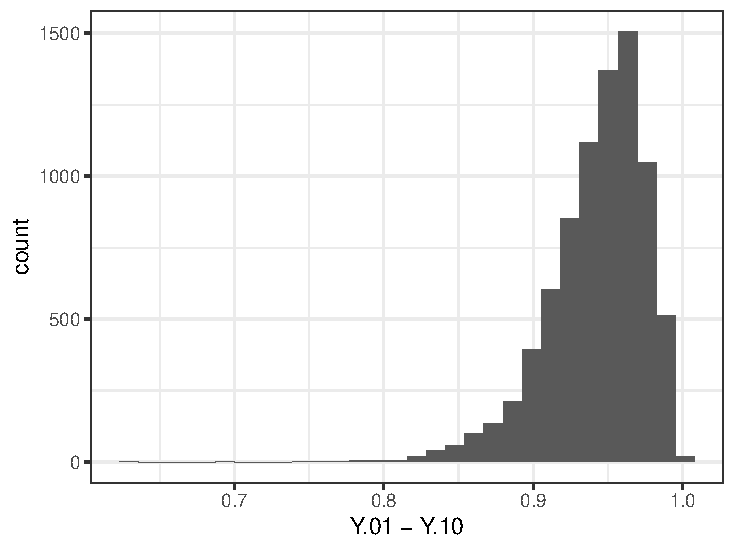
\includegraphics[width=0.6\textwidth,height=\textheight]{paper_files/figure-pdf/fig-posterior-dist-1.pdf}

}

\caption{\label{fig-posterior-dist}Posterior on `Probability \(Y\) is
increasing in \(X\)'}

\end{figure}

\FloatBarrier

\hypertarget{query-distribution}{%
\subsubsection{Query distribution}\label{query-distribution}}

It is generally useful to use causal syntax to define the query and
calculate the query with respect to the prior or posterior probability
distributions.

This can be done for a list of queries using
\texttt{query\_distribution()} function:

\begin{verbatim}
R> make_model("X -> Y") |> 
+  query_distribution(
+    query = list(increasing = "(Y[X=1] > Y[X=0])"), 
+    using = "priors") |>
+  ggplot(aes(increasing)) + geom_histogram() + theme_bw()
\end{verbatim}

\begin{figure}[t]

{\centering \includegraphics[width=0.6\textwidth,height=\textheight]{paper_files/figure-pdf/fig-query-dist-1.pdf}

}

\caption{\label{fig-query-dist}Prior on 'Probability \(Y\) is increasing
in \(X\)'}

\end{figure}

\texttt{query\_distribution()} can also be used when one is interested
in assessing the value of a query for a \emph{particular case}. In a
sense this is equivalent to posing a conditional query, querying
conditional on values in a case. For instance we might consult our
posterior lipids model and ask about the effect of \(X\) on \(Y\) for a
case in which \(Z=1\), \(X=1\) and \(Y=1\).

\begin{verbatim}
R> lipids_model |>
+    query_model(query = "Y[X=1] - Y[X=0]",
+                given = c("X==1 & Y==1 & Z==1"),
+                using = "posteriors")
\end{verbatim}

\hypertarget{tbl-case-level-query}{}
\begin{table}[!h]
\caption{\label{tbl-case-level-query}Case Level Query Example. }\tabularnewline

\centering
\resizebox{\linewidth}{!}{
\begin{tabular}{cccccc}
\toprule
query & given & mean & sd & cred.low & cred.high\\
\midrule
Y[X=1] - Y[X=0] & X==1 \& Y==1 \& Z==1 & 0.95 & 0.04 & 0.87 & 1\\
\bottomrule
\end{tabular}}
\end{table}

The answer we get in Table~\ref{tbl-case-level-query} is what we now
believe for all cases in which \(Z=1, X=1\) and \(Y=1\). It is in fact
the expected average effect among cases with this data type and so this
expectation has an uncertainty attached to it.

Subtly though this is, in principle, different to what we would infer
for a ``new case'' that we wonder about. When inquiring about a new
case, the case level query \emph{updates} on the given information
observed in the new case. The resulting inference can be different to
the inference that would be made from the posterior \emph{given} the
features of the case. If \texttt{case\_level\ =\ TRUE} is specified,
this new case level inference is calculated. For a query \(Q\) and given
\(D\) this returns the value
\(\frac{\int\pi(Q \& D | \lambda_i)p(\lambda_i)d\lambda_i}{\int\pi(D | \lambda_i)p(\lambda_i)d\lambda_i}\)
which may differ from the mean of the distribution
\(\frac{\pi(Q \& D | \lambda)}{\pi(D | \lambda)}\),
\(\int \frac{\pi(Q \& D | \lambda_i)}{\pi(D | \lambda_i)} p(\lambda_i)d\lambda_i\).

To illustrate, consider a model for which we are quite sure that \(X\)
causes \(Y\) but we do not know whether it works through two positive
effects or two negative effects.

Thus we do not know if \(M=0\) would suggest an effect or no effect. If
asked what we would infer for a case that had \(M=0\) we would not know
whether \(M=0\) information is consistent with a positive effect or not.
However if provided with a randomly sampled case and learn that it has
\(M=0\), then we update about the causal model and infer that there is
an effect in this case (but that there would not be were \(M=1\)). The
results are in Table~\ref{tbl-case-level}. Note that the case level
query returns a single number and no posterior standard deviation: this
is the belief about the (new) case in question. The non case case level
query summarizes the posterior distribution over cases with this data.

\begin{verbatim}
R>  make_model("X -> M -> Y") |>
+  update_model(data.frame(X = rep(0:1, 8), Y = rep(0:1, 8)), iter = 10000) |> 
+  query_model(
+    query = "Y[X=1] > Y[X=0]",
+    given = "X==1 & Y==1 & M==1",
+    using = "posteriors",
+    case_level = c(TRUE, FALSE))
\end{verbatim}

\hypertarget{tbl-case-level}{}
\begin{longtable}{ccccc}
\caption{\label{tbl-case-level}Results for a case level query. }\tabularnewline

\toprule
query & given & case\_level & mean & sd\\
\midrule
Y[X=1] > Y[X=0] & X==1 \& Y==1 \& M==1 & TRUE & 0.67 & NA\\
Y[X=1] > Y[X=0] & X==1 \& Y==1 \& M==1 & FALSE & 0.43 & 0.33\\
\bottomrule
\end{longtable}

\hypertarget{batch-queries}{%
\subsubsection{Batch queries}\label{batch-queries}}

The function \texttt{query\_model()} is perhaps the most important
function for querying models. The function takes as input a list of
models, causal queries, and conditions (\texttt{given}), calculates
population or case level estimands given prior or posterior
distributions and reports summaries of these distributions. The result
is a data frame that can be displayed as a table or used for graphing.

Table~\ref{tbl-batch-query} shows output from a single call to
\texttt{query\_model}.

\begin{verbatim}
R> models <- list(
+ `1` = make_model("X -> Y"),
+ `2` = make_model("X -> Y") |> set_restrictions("Y[X=1] < Y[X=0]")
+ )
R> 
R> query_model(
+  models,
+  query = list(ATE = "Y[X=1] - Y[X=0]", 
+               POS = "Y[X=1] > Y[X=0]"),
+  given = c(TRUE,  "Y==1 & X==1"),
+  case_level = c(FALSE, TRUE),
+  using = c("parameters", "priors"),
+  expand_grid = TRUE)
\end{verbatim}

\hypertarget{tbl-batch-query}{}
\begin{longtable}{ccccccc}
\caption{\label{tbl-batch-query}Results for Two Queries on Two Models. }\tabularnewline

\toprule
model & query & given & using & case\_level & mean & sd\\
\midrule
1 & ATE & - & parameters & FALSE & 0.00 & NA\\
2 & ATE & - & parameters & FALSE & 0.33 & NA\\
1 & ATE & - & priors & FALSE & -0.01 & 0.32\\
2 & ATE & - & priors & FALSE & 0.33 & 0.24\\
1 & ATE & Y==1 \& X==1 & parameters & FALSE & 0.50 & NA\\
2 & ATE & Y==1 \& X==1 & parameters & FALSE & 0.50 & NA\\
1 & ATE & Y==1 \& X==1 & priors & FALSE & 0.50 & 0.29\\
2 & ATE & Y==1 \& X==1 & priors & FALSE & 0.50 & 0.29\\
1 & POS & - & parameters & FALSE & 0.25 & NA\\
2 & POS & - & parameters & FALSE & 0.33 & NA\\
1 & POS & - & priors & FALSE & 0.25 & 0.20\\
2 & POS & - & priors & FALSE & 0.33 & 0.24\\
1 & POS & Y==1 \& X==1 & parameters & FALSE & 0.50 & NA\\
2 & POS & Y==1 \& X==1 & parameters & FALSE & 0.50 & NA\\
1 & POS & Y==1 \& X==1 & priors & FALSE & 0.50 & 0.29\\
2 & POS & Y==1 \& X==1 & priors & FALSE & 0.50 & 0.29\\
1 & ATE & - & parameters & TRUE & 0.00 & NA\\
2 & ATE & - & parameters & TRUE & 0.33 & NA\\
1 & ATE & - & priors & TRUE & -0.01 & NA\\
2 & ATE & - & priors & TRUE & 0.33 & NA\\
1 & ATE & Y==1 \& X==1 & parameters & TRUE & 0.50 & NA\\
2 & ATE & Y==1 \& X==1 & parameters & TRUE & 0.50 & NA\\
1 & ATE & Y==1 \& X==1 & priors & TRUE & 0.51 & NA\\
2 & ATE & Y==1 \& X==1 & priors & TRUE & 0.50 & NA\\
1 & POS & - & parameters & TRUE & 0.25 & NA\\
2 & POS & - & parameters & TRUE & 0.33 & NA\\
1 & POS & - & priors & TRUE & 0.25 & NA\\
2 & POS & - & priors & TRUE & 0.33 & NA\\
1 & POS & Y==1 \& X==1 & parameters & TRUE & 0.50 & NA\\
2 & POS & Y==1 \& X==1 & parameters & TRUE & 0.50 & NA\\
1 & POS & Y==1 \& X==1 & priors & TRUE & 0.51 & NA\\
2 & POS & Y==1 \& X==1 & priors & TRUE & 0.50 & NA\\
\bottomrule
\end{longtable}

The \texttt{stats} argument lets users specify alternative summary
statistics. The \texttt{expand\_grid} argument lets users specify
whether all combinations of list elements should be generated.

\FloatBarrier

\hypertarget{computational-details-and-software-requirements}{%
\section*{Computational details and software
requirements}\label{computational-details-and-software-requirements}}
\addcontentsline{toc}{section}{Computational details and software
requirements}

\begin{longtable}[]{@{}
  >{\raggedleft\arraybackslash}p{(\columnwidth - 2\tabcolsep) * \real{0.3000}}
  >{\raggedright\arraybackslash}p{(\columnwidth - 2\tabcolsep) * \real{0.7000}}@{}}
\toprule\noalign{}
\endhead
\bottomrule\noalign{}
\endlastfoot
Version & \begin{minipage}[t]{\linewidth}\raggedright
\begin{itemize}
\tightlist
\item
  1.0.1
\end{itemize}
\end{minipage} \\
Availability & \begin{minipage}[t]{\linewidth}\raggedright
\begin{itemize}
\tightlist
\item
  Stable Release:
  \url{https://cran.rstudio.com/web/packages/CausalQueries/index.html}
\item
  Development:
  \url{https://github.com/integrated-inferences/CausalQueries}
\end{itemize}
\end{minipage} \\
Issues & \begin{minipage}[t]{\linewidth}\raggedright
\begin{itemize}
\tightlist
\item
  \url{https://github.com/integrated-inferences/CausalQueries/issues}
\end{itemize}
\end{minipage} \\
Operating Systems & \begin{minipage}[t]{\linewidth}\raggedright
\begin{itemize}
\tightlist
\item
  Linux
\item
  MacOS
\item
  Windows
\end{itemize}
\end{minipage} \\
Testing Environments OS & \begin{minipage}[t]{\linewidth}\raggedright
\begin{itemize}
\tightlist
\item
  Ubuntu 22.04.2
\item
  Debian 12.2
\item
  MacOS
\item
  Windows
\end{itemize}
\end{minipage} \\
Testing Environments R & \begin{minipage}[t]{\linewidth}\raggedright
\begin{itemize}
\tightlist
\item
  R 4.3.1
\item
  R 4.3.0
\item
  R 4.2.3
\item
  r-devel
\end{itemize}
\end{minipage} \\
R Version & \begin{minipage}[t]{\linewidth}\raggedright
\begin{itemize}
\tightlist
\item
  R(\textgreater= 3.4.0)
\end{itemize}
\end{minipage} \\
Compiler & \begin{minipage}[t]{\linewidth}\raggedright
\begin{itemize}
\tightlist
\item
  either of the below or similar:
\item
  g++
\item
  clang++
\end{itemize}
\end{minipage} \\
Stan requirements & \begin{minipage}[t]{\linewidth}\raggedright
\begin{itemize}
\tightlist
\item
  inline
\item
  Rcpp (\textgreater= 0.12.0)
\item
  RcppEigen (\textgreater= 0.3.3.3.0)
\item
  RcppArmadillo (\textgreater= 0.12.6.4.0)
\item
  RcppParallel (\textgreater= 5.1.4)
\item
  BH (\textgreater= 1.66.0)
\item
  StanHeaders (\textgreater= 2.26.0)
\item
  rstan (\textgreater= 2.26.0)
\end{itemize}
\end{minipage} \\
R-Packages Depends & \begin{minipage}[t]{\linewidth}\raggedright
\begin{itemize}
\tightlist
\item
  dplyr
\item
  methods
\end{itemize}
\end{minipage} \\
R-Packages Imports & \begin{minipage}[t]{\linewidth}\raggedright
\begin{itemize}
\tightlist
\item
  dagitty (\textgreater= 0.3-1)
\item
  dirmult (\textgreater= 0.1.3-4)
\item
  stats (\textgreater= 4.1.1)
\item
  rlang (\textgreater= 0.2.0)
\item
  rstan (\textgreater= 2.26.0)
\item
  rstantools (\textgreater= 2.0.0)
\item
  stringr (\textgreater= 1.4.0)
\item
  ggdag (\textgreater= 0.2.4)
\item
  latex2exp (\textgreater= 0.9.4)
\item
  ggplot2 (\textgreater= 3.3.5)
\item
  lifecycle (\textgreater= 1.0.1)
\end{itemize}
\end{minipage} \\
\end{longtable}

The results in this paper were obtained using
\proglang{R}\textasciitilde3.4.1 with the
\pkg{MASS}\textasciitilde7.3.47 package. \proglang{R} itself and all
packages used are available from the Comprehensive \proglang{R} Archive
Network (CRAN) at \url{https://CRAN.R-project.org/}.

\hypertarget{benchmarks}{%
\section{Benchmarks}\label{benchmarks}}

We present a brief summary of model updating benchmarks. Benchmark 1 we
considers the effect of model complexity on updating time. Benchmark 2
considers the effect of data size on model complexity. We run 4 parallel
chains for each model.

\begin{longtable}[]{@{}
  >{\centering\arraybackslash}p{(\columnwidth - 4\tabcolsep) * \real{0.4000}}
  >{\centering\arraybackslash}p{(\columnwidth - 4\tabcolsep) * \real{0.3000}}
  >{\centering\arraybackslash}p{(\columnwidth - 4\tabcolsep) * \real{0.3000}}@{}}
\toprule\noalign{}
\begin{minipage}[b]{\linewidth}\centering
Model
\end{minipage} & \begin{minipage}[b]{\linewidth}\centering
Number of Model Parameters
\end{minipage} & \begin{minipage}[b]{\linewidth}\centering
\texttt{update\_model()} Runt-Time (seconds)
\end{minipage} \\
\midrule\noalign{}
\endhead
\bottomrule\noalign{}
\endlastfoot
\(X1 \rightarrow Y\) & 6 & 10.85 \\
\(X1 \rightarrow Y \leftarrow X2\) & 20 & 15.79 \\
\(X1 \rightarrow Y \leftarrow X2; X3 \rightarrow Y\) & 262 & 77.56 \\
\end{longtable}

\begin{longtable}[]{@{}
  >{\centering\arraybackslash}p{(\columnwidth - 4\tabcolsep) * \real{0.4000}}
  >{\centering\arraybackslash}p{(\columnwidth - 4\tabcolsep) * \real{0.3000}}
  >{\centering\arraybackslash}p{(\columnwidth - 4\tabcolsep) * \real{0.3000}}@{}}
\toprule\noalign{}
\begin{minipage}[b]{\linewidth}\centering
Model
\end{minipage} & \begin{minipage}[b]{\linewidth}\centering
Number of Observations
\end{minipage} & \begin{minipage}[b]{\linewidth}\centering
\texttt{update\_model()} Runt-Time (seconds)
\end{minipage} \\
\midrule\noalign{}
\endhead
\bottomrule\noalign{}
\endlastfoot
\(X1 \rightarrow Y\) & 10 & 9.04 \\
\(X1 \rightarrow Y\) & 100 & 9.31 \\
\(X1 \rightarrow Y\) & 1000 & 10.56 \\
\(X1 \rightarrow Y\) & 10000 & 14.57 \\
\(X1 \rightarrow Y\) & 100000 & 17.25 \\
\end{longtable}

While model updating is fundamentally a \(O(N)\) time complexity
operation with respect to model and data size; the exponential growth of
the parameter space with increasing model complexity places limits on
feasible computability without further recourse to specialized methods
for handling large causal models.

\hypertarget{acknowledgments}{%
\section*{Acknowledgments}\label{acknowledgments}}
\addcontentsline{toc}{section}{Acknowledgments}

\begin{tcolorbox}[enhanced jigsaw, opacityback=0, breakable, colback=white, bottomrule=.15mm, toprule=.15mm, arc=.35mm, rightrule=.15mm, leftrule=.75mm, left=2mm]

The approach to generating a generic function to create Stan code that
can take data from arbitrary models was developed in key contributions
by \href{http://jasper-cooper.com/}{Jasper Cooper} and
\href{http://gsyunyaev.com/}{Georgiy Syunyaev}.
\href{https://lilymedina.github.io/}{Lily Medina} did magical work
pulling it all together and developing approaches to characterizing
confounding and defining estimands. Clara Bicalho helped figure out the
syntax for causal statements. Julio Solis made many key contributions
figuring out how to simplify the specification of priors. Merlin
Heidemanns figured out the \texttt{rstantools} integration and made
myriad code improvements. Till Tietz revamped the entire package and
improved every part of it.

\end{tcolorbox}

\hypertarget{references}{%
\section*{References}\label{references}}
\addcontentsline{toc}{section}{References}

\renewcommand{\bibsection}{}
\bibliography{supp/cq_jss.bib}

\newpage{}

\hypertarget{sec-techdetails}{%
\section*{More technical details}\label{sec-techdetails}}
\addcontentsline{toc}{section}{More technical details}

\hypertarget{appendix-stan-code}{%
\section{Appendix: Stan code}\label{appendix-stan-code}}

Updating is performed using Stan model. The data provided to Stan is
generated by the internal function \texttt{prep\_stan\_data()} which
returns a list of objects that Stan expects to receive. The code for the
Stan model is show below. After defining a helper function the code
starts with a block declaring what input data is to be expected. Then
there is a characterization of parameters and the transformed
parameters. Then the likelihoods and priors are provided. At the end
there is a block for generated quantities which can be used to append a
posterior distribution of causal types to the model.

\begin{verbatim}
functions{
  row_vector col_sums(matrix X) {
    row_vector[cols(X)] s ;
    s = rep_row_vector(1, rows(X)) * X ;
    return s ;
  }
}
data {
int<lower=1> n_params;
int<lower=1> n_paths;
int<lower=1> n_types;
int<lower=1> n_param_sets;
int<lower=1> n_nodes;
array[n_param_sets] int<lower=1> n_param_each;
int<lower=1> n_data;
int<lower=1> n_events;
int<lower=1> n_strategies;
int<lower=0, upper=1> keep_transformed;
vector<lower=0>[n_params] lambdas_prior;
array[n_param_sets] int<lower=1> l_starts;
array[n_param_sets] int<lower=1> l_ends;
array[n_nodes] int<lower=1> node_starts;
array[n_nodes] int<lower=1> node_ends;
array[n_strategies] int<lower=1> strategy_starts;
array[n_strategies] int<lower=1> strategy_ends;
matrix[n_params, n_types] P;
matrix[n_params, n_paths] parmap;
matrix[n_paths, n_data] map;
matrix<lower=0,upper=1>[n_events,n_data] E;
array[n_events] int<lower=0> Y;
}
parameters {
vector<lower=0>[n_params - n_param_sets] gamma;
}
transformed parameters {
vector<lower=0, upper=1>[n_params] lambdas;
vector<lower=1>[n_param_sets] sum_gammas;
matrix[n_params, n_paths] parlam;
matrix[n_nodes, n_paths] parlam2;
vector<lower=0, upper=1>[n_paths] w_0;
vector<lower=0, upper=1>[n_data] w;
vector<lower=0, upper=1>[n_events] w_full;
// Cases in which a parameter set has only one value need special handling
// they have no gamma components and sum_gamma needs to be made manually
for (i in 1:n_param_sets) {
  if (l_starts[i] >= l_ends[i]) {
    sum_gammas[i] = 1;
    // syntax here to return unity as a vector
    lambdas[l_starts[i]] = lambdas_prior[1]/lambdas_prior[1];
    }
  else if (l_starts[i] < l_ends[i]) {
    sum_gammas[i] =
    1 + sum(gamma[(l_starts[i] - (i-1)):(l_ends[i] - i)]);
    lambdas[l_starts[i]:l_ends[i]] =
    append_row(1, gamma[(l_starts[i] - (i-1)):(l_ends[i] - i)]) /
      sum_gammas[i];
    }
  }
// Mapping from parameters to data types
// (usual case): [n_par * n_data] * [n_par * n_data]
parlam  = rep_matrix(lambdas, n_paths) .* parmap;
// Sum probability over nodes on each path
for (i in 1:n_nodes) {
 parlam2[i,] = col_sums(parlam[(node_starts[i]):(node_ends[i]),]);
 }
// then take product  to get probability of data type on path
for (i in 1:n_paths) {
  w_0[i] = prod(parlam2[,i]);
 }
 // last (if confounding): map to n_data columns instead of n_paths
 w = map'*w_0;
  // Extend/reduce to cover all observed data types
 w_full = E * w;
}
model {
// Dirichlet distributions (earlier versions used gamma)
for (i in 1:n_param_sets) {
  target += dirichlet_lpdf(lambdas[l_starts[i]:l_ends[i]]  |
    lambdas_prior[l_starts[i] :l_ends[i]]);
  target += -n_param_each[i] * log(sum_gammas[i]);
 }
// Multinomials
// Note with censoring event_probabilities might not sum to 1
for (i in 1:n_strategies) {
  target += multinomial_lpmf(
  Y[strategy_starts[i]:strategy_ends[i]] |
    w_full[strategy_starts[i]:strategy_ends[i]]/
     sum(w_full[strategy_starts[i]:strategy_ends[i]]));
 }
}
// Option to export distribution of causal types
generated quantities{
vector[n_types] prob_of_types;
if (keep_transformed == 1){
for (i in 1:n_types) {
   prob_of_types[i] = prod(P[, i].*lambdas + 1 - P[,i]);
}}
 if (keep_transformed == 0){
    prob_of_types = rep_vector(1, n_types);
 }
}
\end{verbatim}




\end{document}
